%!TEX root = ../thesis.tex
% ******************************* Thesis Appendix C ********************************

\chapter{}
\ifpdf
\graphicspath{{chapter-pmssm/Figs/Raster/}{chapter-pmssm/Figs/PDF/}{chapter-pmssm/Figs/}}
\else
\graphicspath{{chapter-pmssm/Figs/Vector/}{chapter-pmssm/Figs/}}
\fi

\section{Phenomenology of the LSP}

In the following, various two-dimensional projections of the parameter space sampled in function of the \gls{lsp} type are shown.

\Cref{fig:lsp_phenomenology_parameters} shows the \gls{lsp} type as a function of the \gls{pmssm} parameters $M_1$, $M_2$, $\mu$ and $\tan\beta$, illustrating the behaviour of the neutralino mass mixing matrix introduced in \cref{ch:gauge_theory}. Models with $\vert M_1\vert < \vert M_2\vert$ and $\vert M_1\vert \ll \vert\mu\vert$ tend to have an \gls{lsp} with dominant bino component, while, in models with $\vert M_2 \vert < \vert M_1 \vert$ and $ \vert M_2 \vert  \ll \vert\mu\vert$, the \gls{lsp} is mostly wino-like. Models where  $\vert\mu\vert\ll \vert M_1 \vert$ and $\vert\mu\vert\ll \vert M_2 \vert$, the \gls{lsp} is mostly higgsino-like. In models with mass parameters in between those edge cases, the \gls{lsp} becomes a mixed state. The parameter $\tan\beta$ does not have a large impact on the \gls{lsp} type within the ranges sampled.

\Cref{fig:impact_electroweakinos_2D_bino_lsp} shows the fraction of models excluded by the \onelepton search in different two-dimensional projections on the electroweakino masses. Only models with a bino-like or wino-like \gls{lsp} are shown in order to highlight the different spectra. No models with a higgsino-like \gls{lsp} are shown since the \onelepton search is not sensitive to such scenarios. Models with a bino-like \gls{lsp} tend to have nearly mass-degenerate $\charg$ and $\neutr$ and are thus close to the canonical simplified model considered in the search. Models with a wino-like \gls{lsp} have nearly mass-degenerate $\charg$ and $\lsp$. In such models, the \onelepton search can become sensitive to $\tilde{\chi}_2^\pm\neutr$ production with subsequent decay $\tilde{\chi}_2^\pm \to h\lsp$.

 \begin{figure}
	\centering
	\begin{subfigure}[b]{0.5\linewidth}
		\centering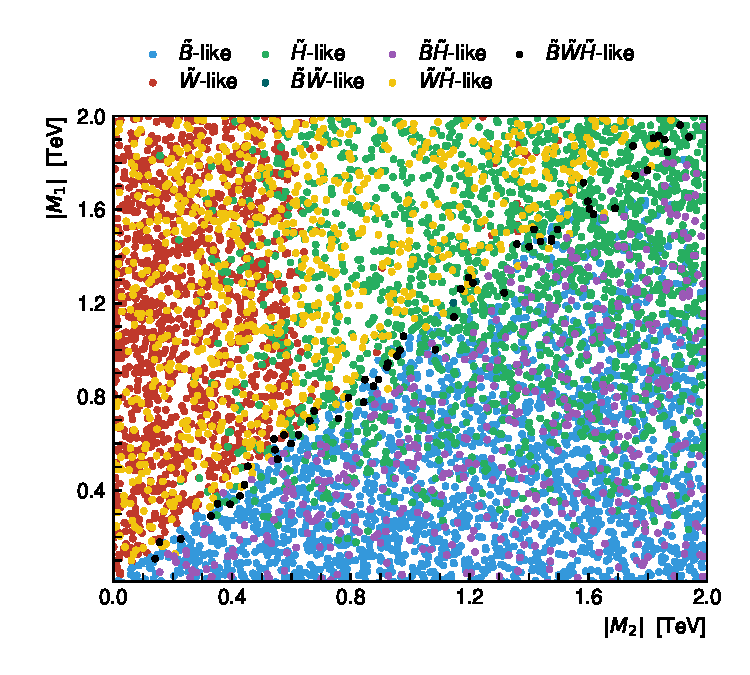
\includegraphics[width=\textwidth]{scatter/lsp_types_M1_M2}
	\end{subfigure}\hfill
	\begin{subfigure}[b]{0.5\linewidth}
		\centering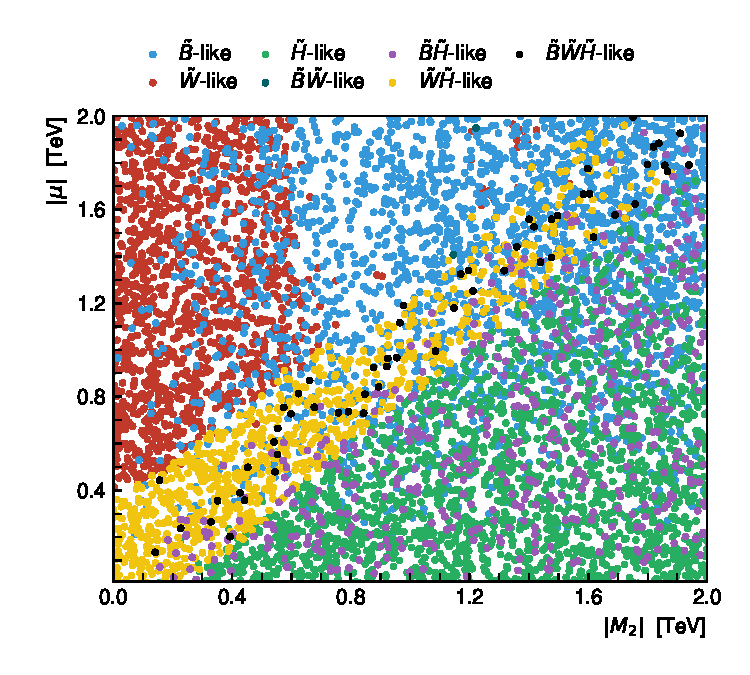
\includegraphics[width=\textwidth]{scatter/lsp_types_mu_M2}
	\end{subfigure}\hfill
	\begin{subfigure}[b]{0.5\linewidth}
		\centering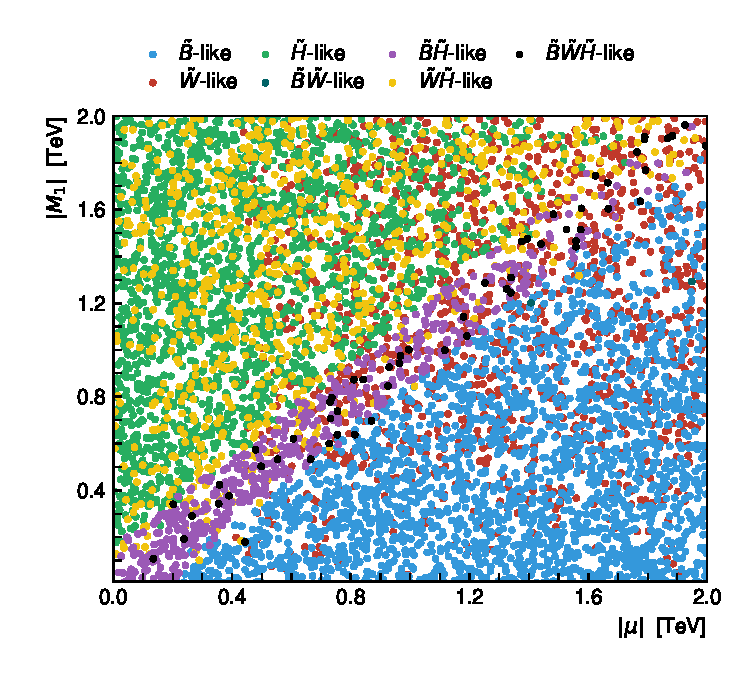
\includegraphics[width=\textwidth]{scatter/lsp_types_mu_M1}
	\end{subfigure}\hfill
	\begin{subfigure}[b]{0.5\linewidth}
		\centering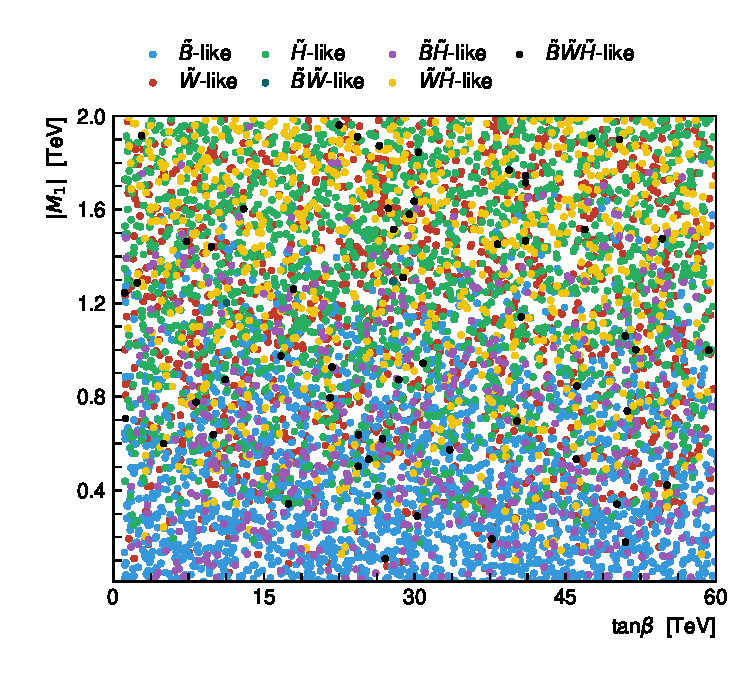
\includegraphics[width=\textwidth]{scatter/lsp_types_tanb_M1}
	\end{subfigure}\hfill
	\caption{Phenomenology of the \gls{lsp} as a function of two-dimensional projections of the \gls{pmssm} parameter space. The parameters $M_1$, $M_2$, $\mu$ and $\tan\beta$ in various projections. Each point in the plots corresponds to a unique \gls{pmssm} model sampled. The colour codes the nature of the \gls{lsp} using the definitions introduced in \cref{sec:lsp_pheno}.}
	\label{fig:lsp_phenomenology_parameters}
\end{figure}


\begin{figure}
	\centering
	\begin{subfigure}[b]{0.5\linewidth}
		\centering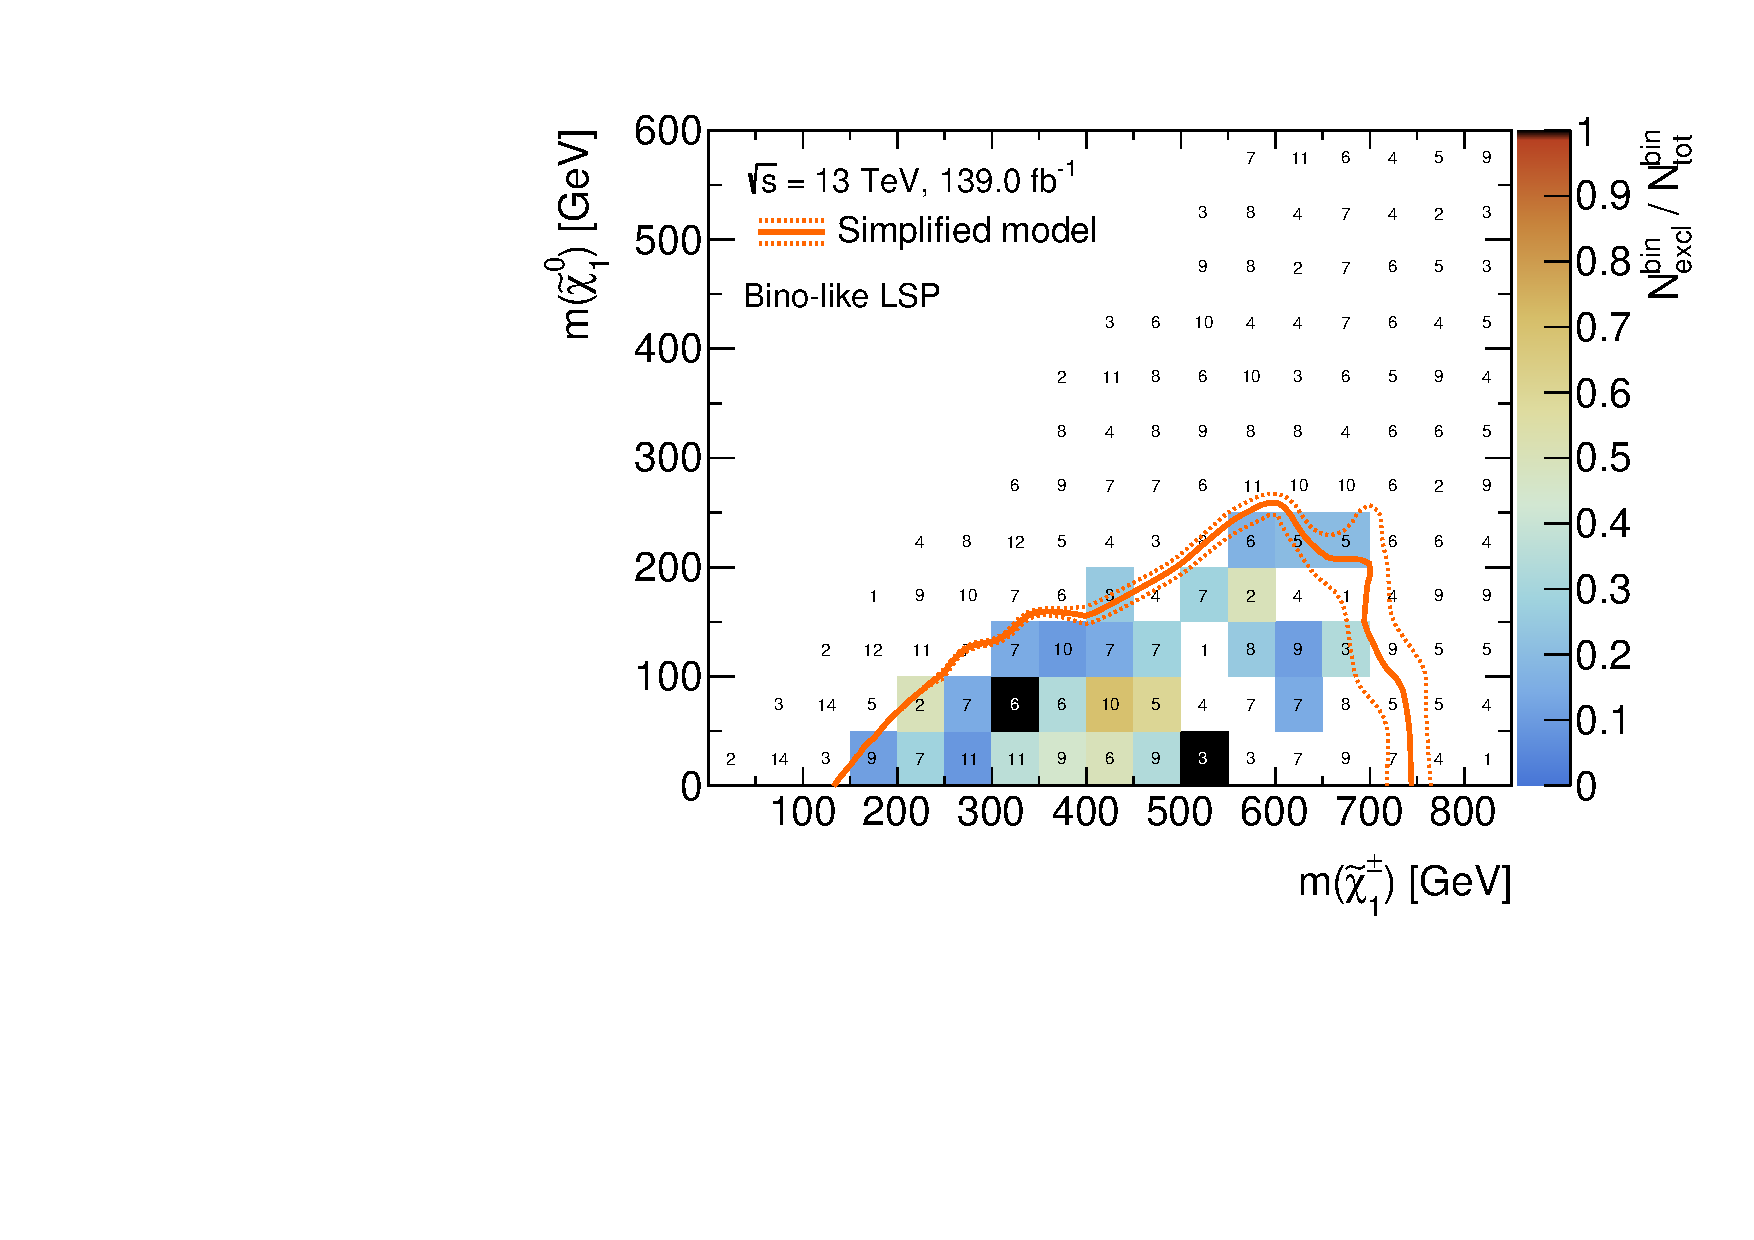
\includegraphics[width=\textwidth]{cut_bino_LSP/mchi1p_mlsp_contour}
	\end{subfigure}\hfill
	\begin{subfigure}[b]{0.5\linewidth}
		\centering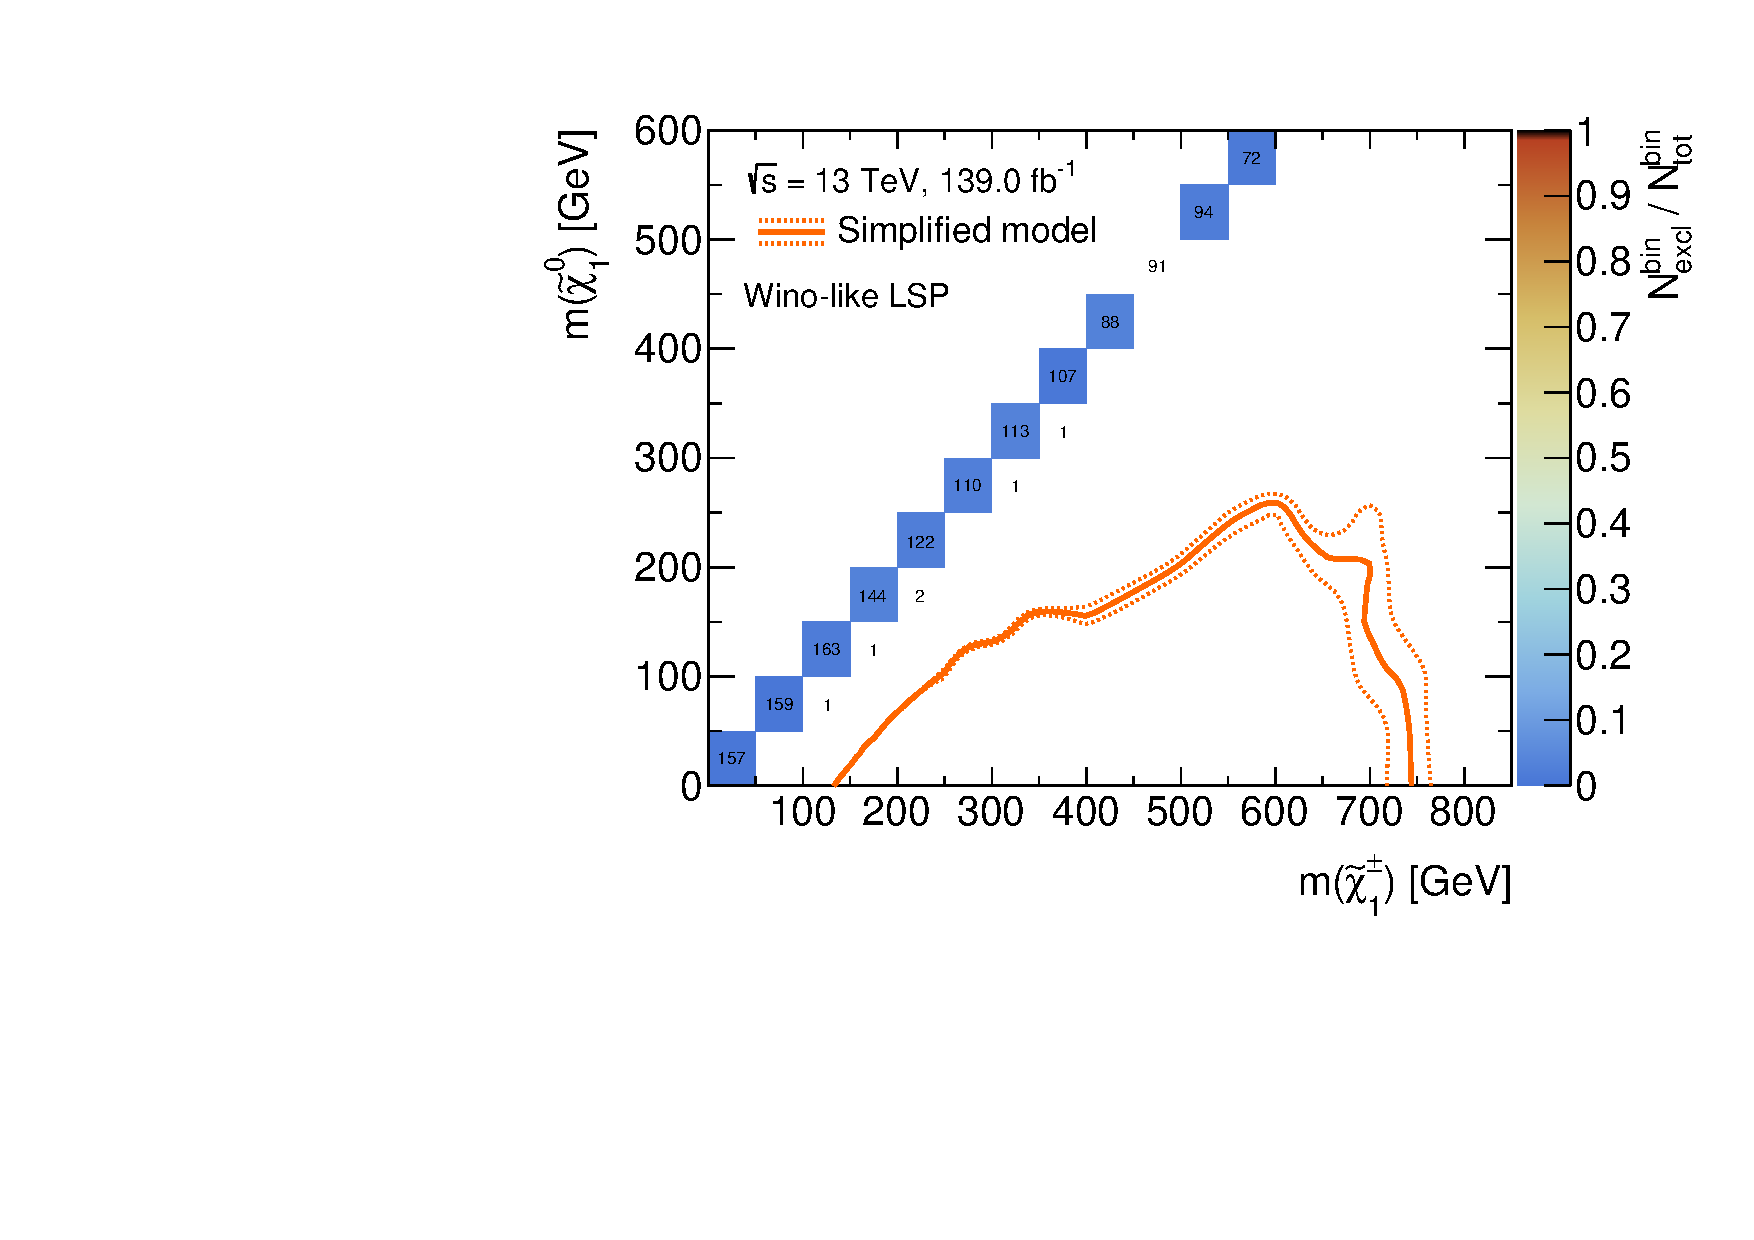
\includegraphics[width=\textwidth]{cut_wino_LSP/mchi1p_mlsp_contour}
	\end{subfigure}\hfill
	
	\begin{subfigure}[b]{0.5\linewidth}
		\centering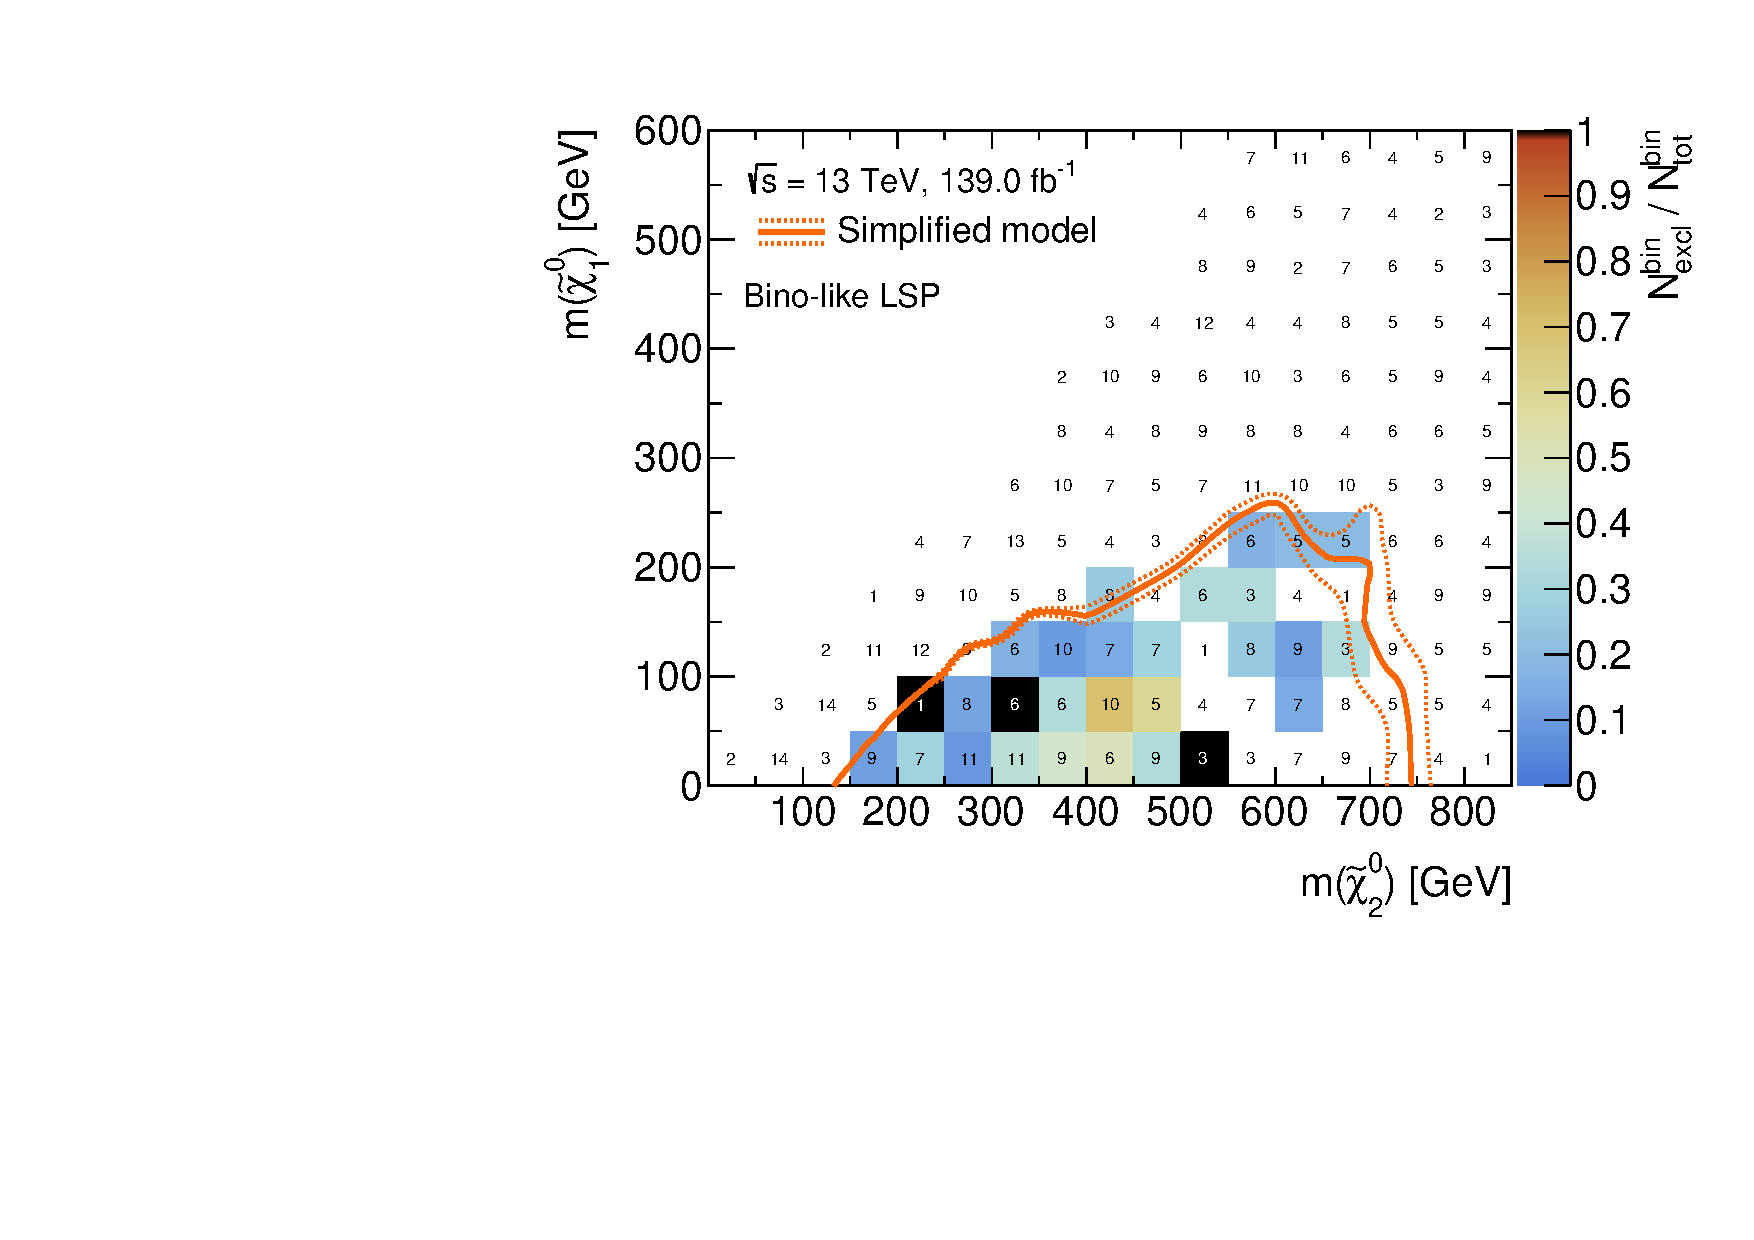
\includegraphics[width=\textwidth]{cut_bino_LSP/mchi20_mlsp_contour}
	\end{subfigure}\hfill
	\begin{subfigure}[b]{0.5\linewidth}
		\centering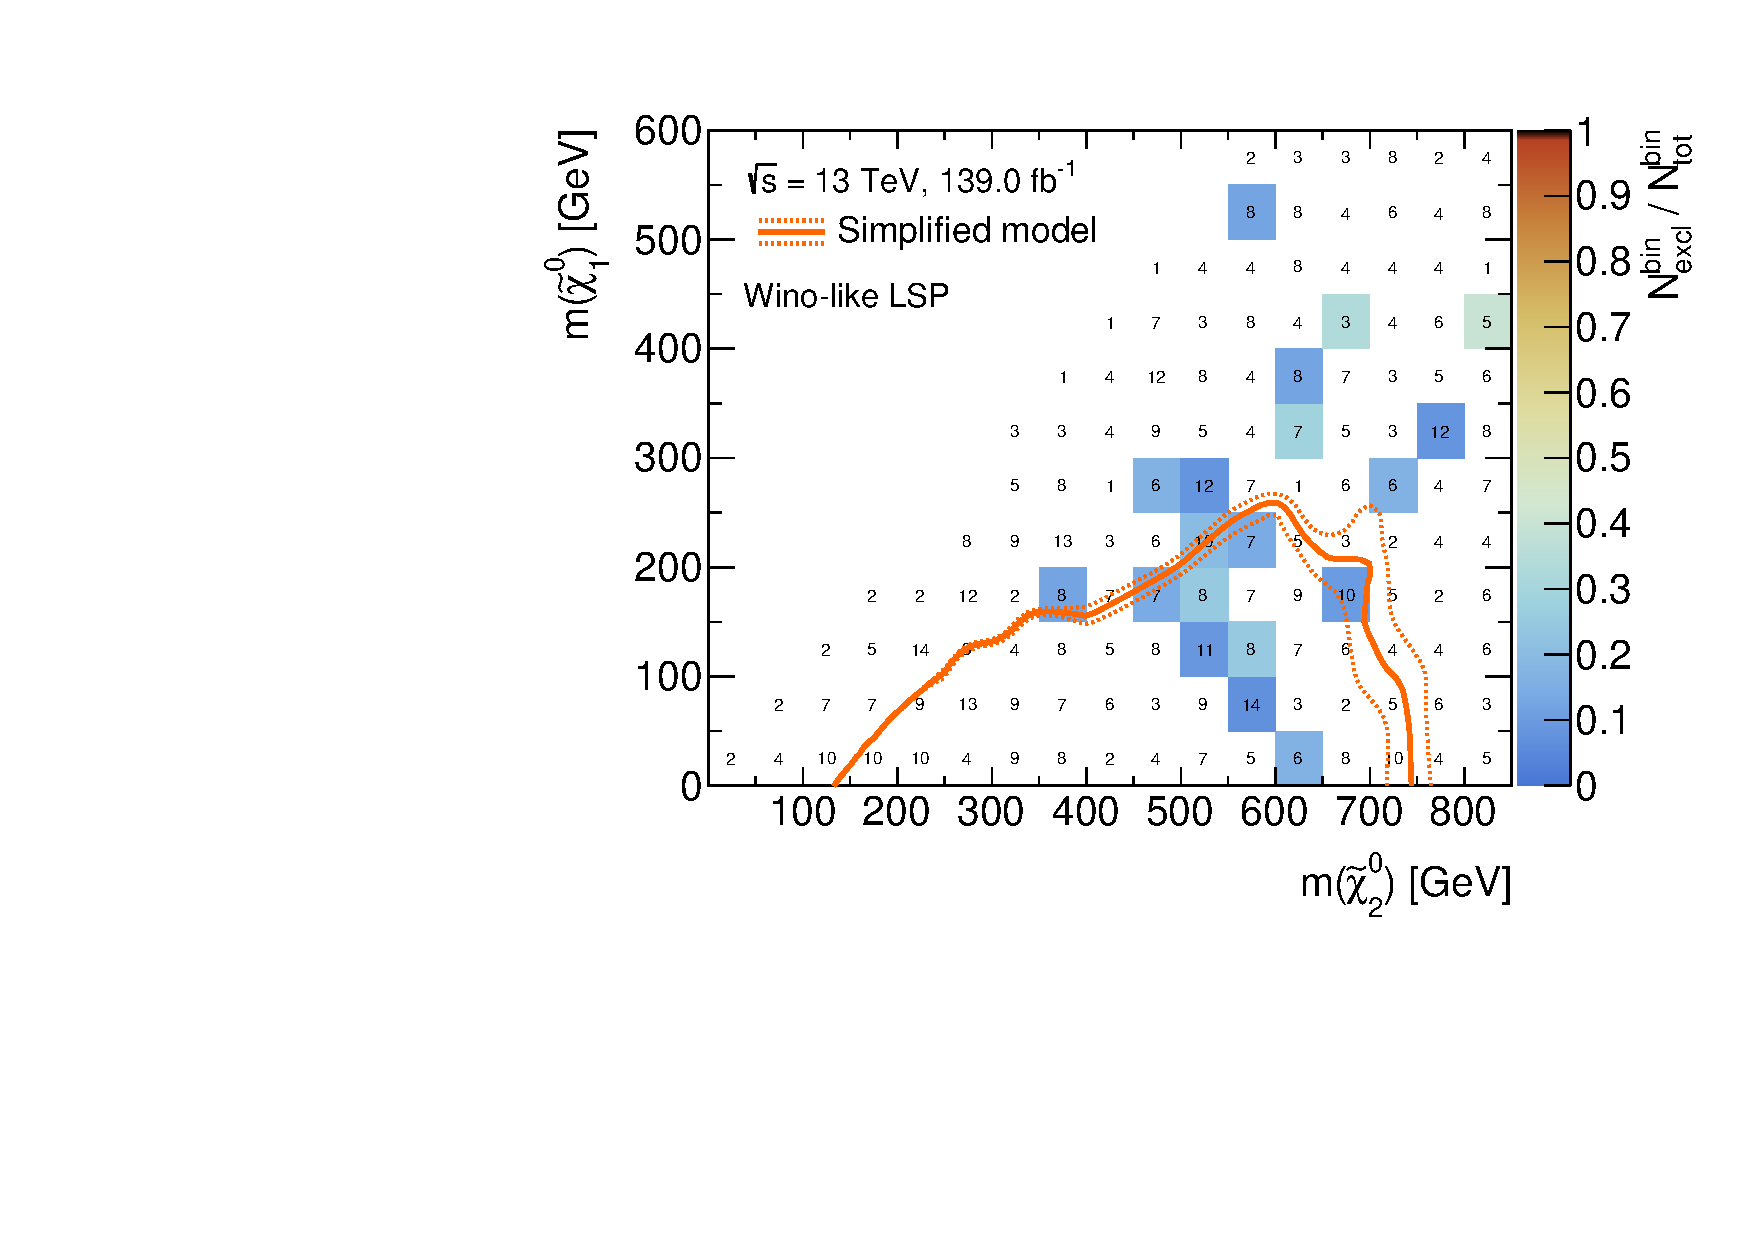
\includegraphics[width=\textwidth]{cut_wino_LSP/mchi20_mlsp_contour}
	\end{subfigure}\hfill
	
	\begin{subfigure}[b]{0.5\linewidth}
		\centering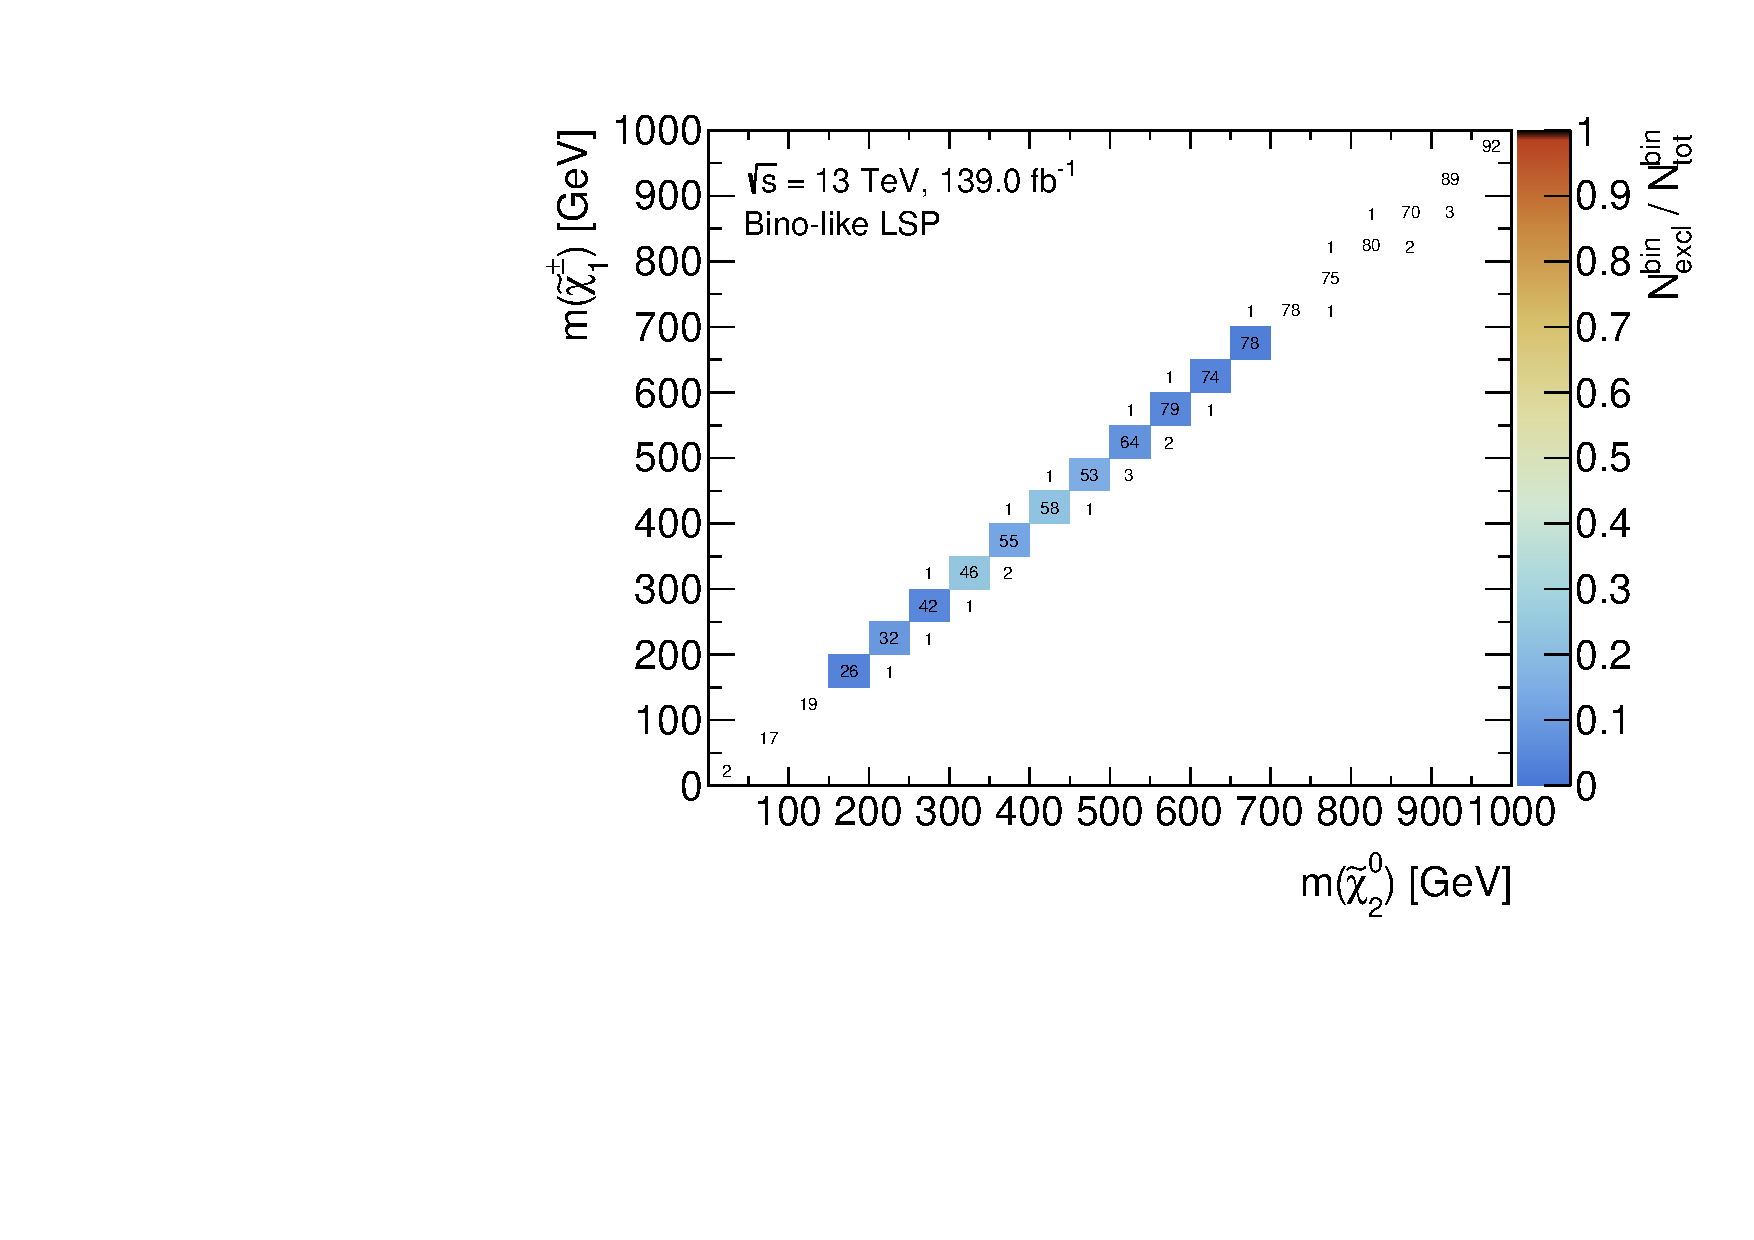
\includegraphics[width=\textwidth]{cut_bino_LSP/mchi1p_mchi20_contour}
	\end{subfigure}\hfill
	\begin{subfigure}[b]{0.5\linewidth}
		\centering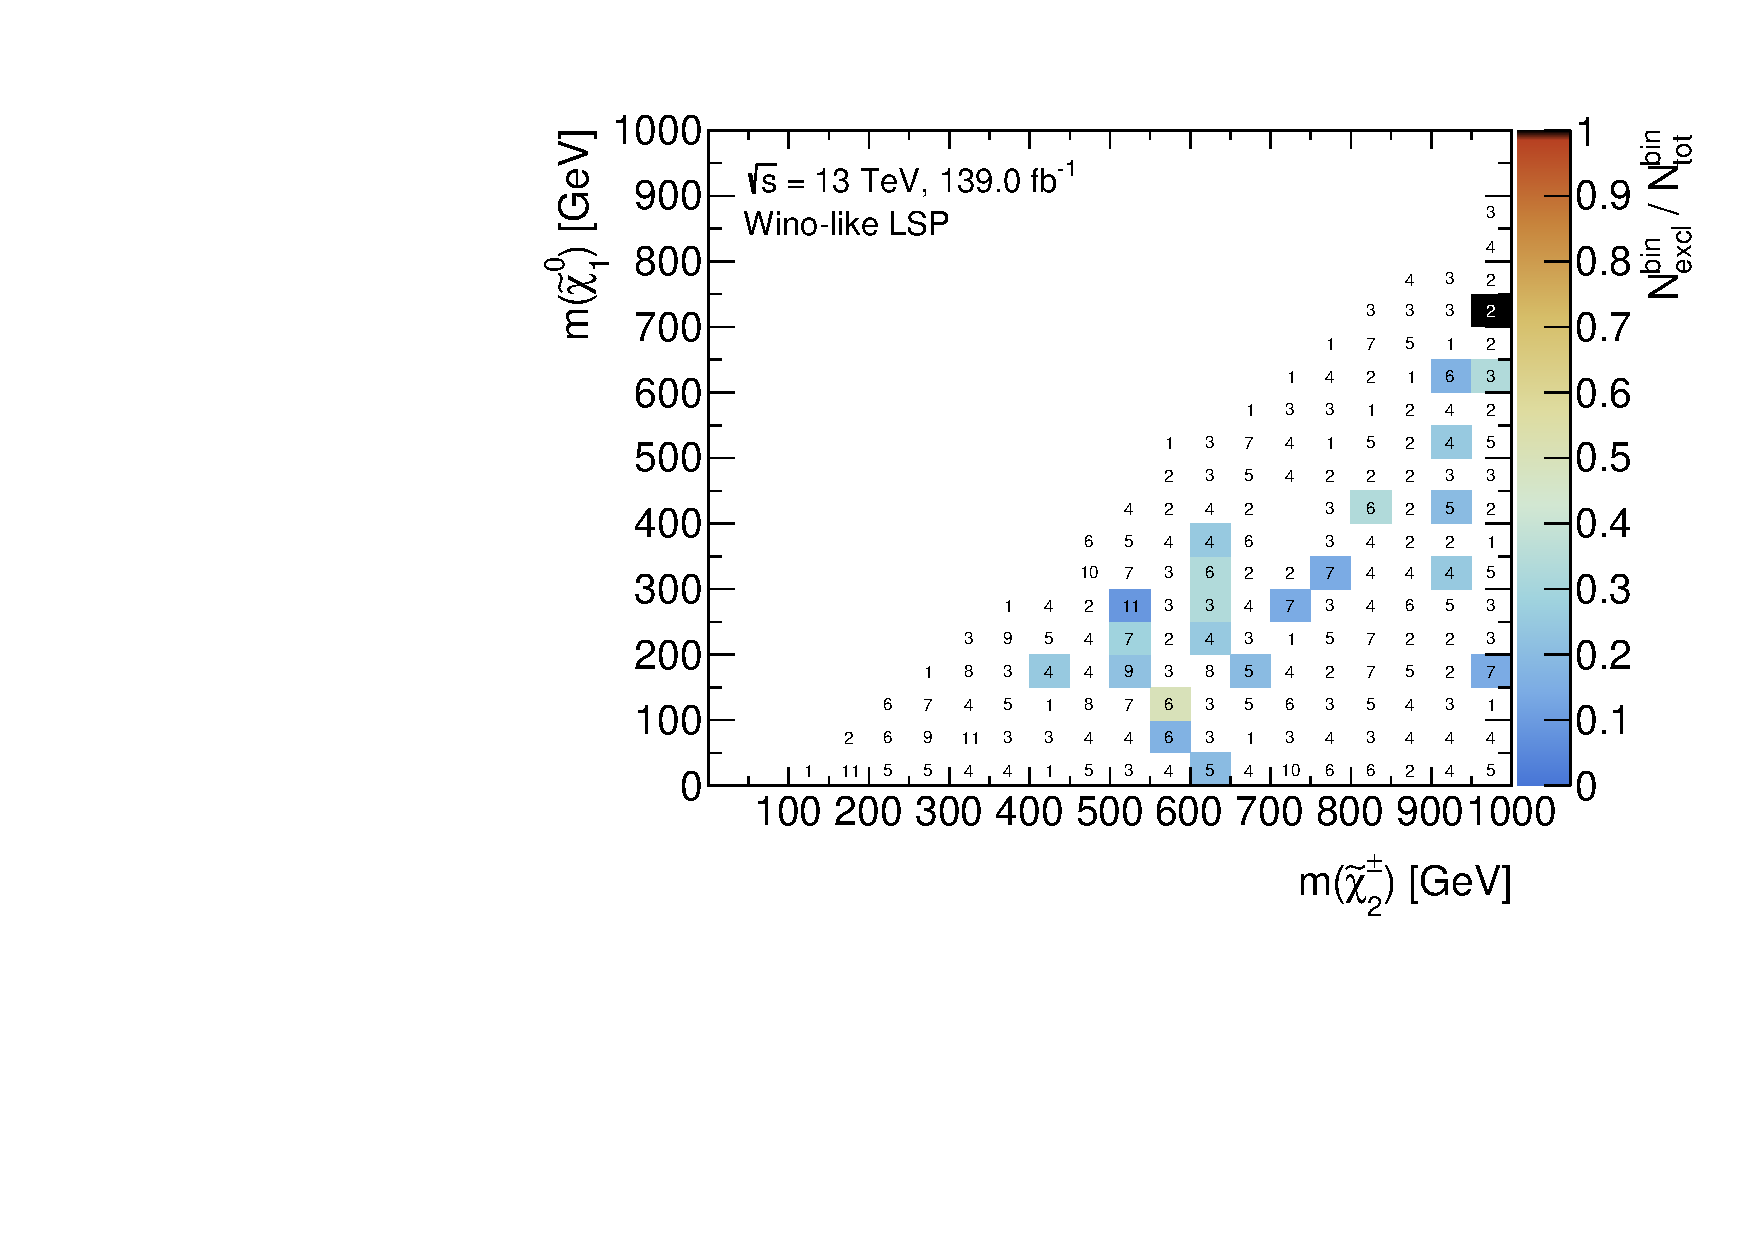
\includegraphics[width=\textwidth]{cut_wino_LSP/mchi10_mchi2p_contour}
	\end{subfigure}\hfill	
	
	\caption{Bin-by-bin fraction of excluded models as a two-dimensional function of the relevant sparticle masses. Only \gls{pmssm} models with a bino-like (wino-like) \gls{lsp} are shown on the left (right). The numbers in the bins correspond to the total number of models sampled falling into the respective bin. The number of models excluded by the \onelepton search is encoded with a colour bar ranging from 0 to 1. Where all models in a given bin are excluded, the bin is coloured in black. Bins without any models excluded are left white. Models are evaluated using the simplified likelihood of the 1-lepton analysis. The simplified model contour is shown in orange.}
	\label{fig:impact_electroweakinos_2D_bino_lsp}
\end{figure}

% \begin{figure}
%	\centering
%	\begin{subfigure}[b]{0.5\linewidth}
%		\centering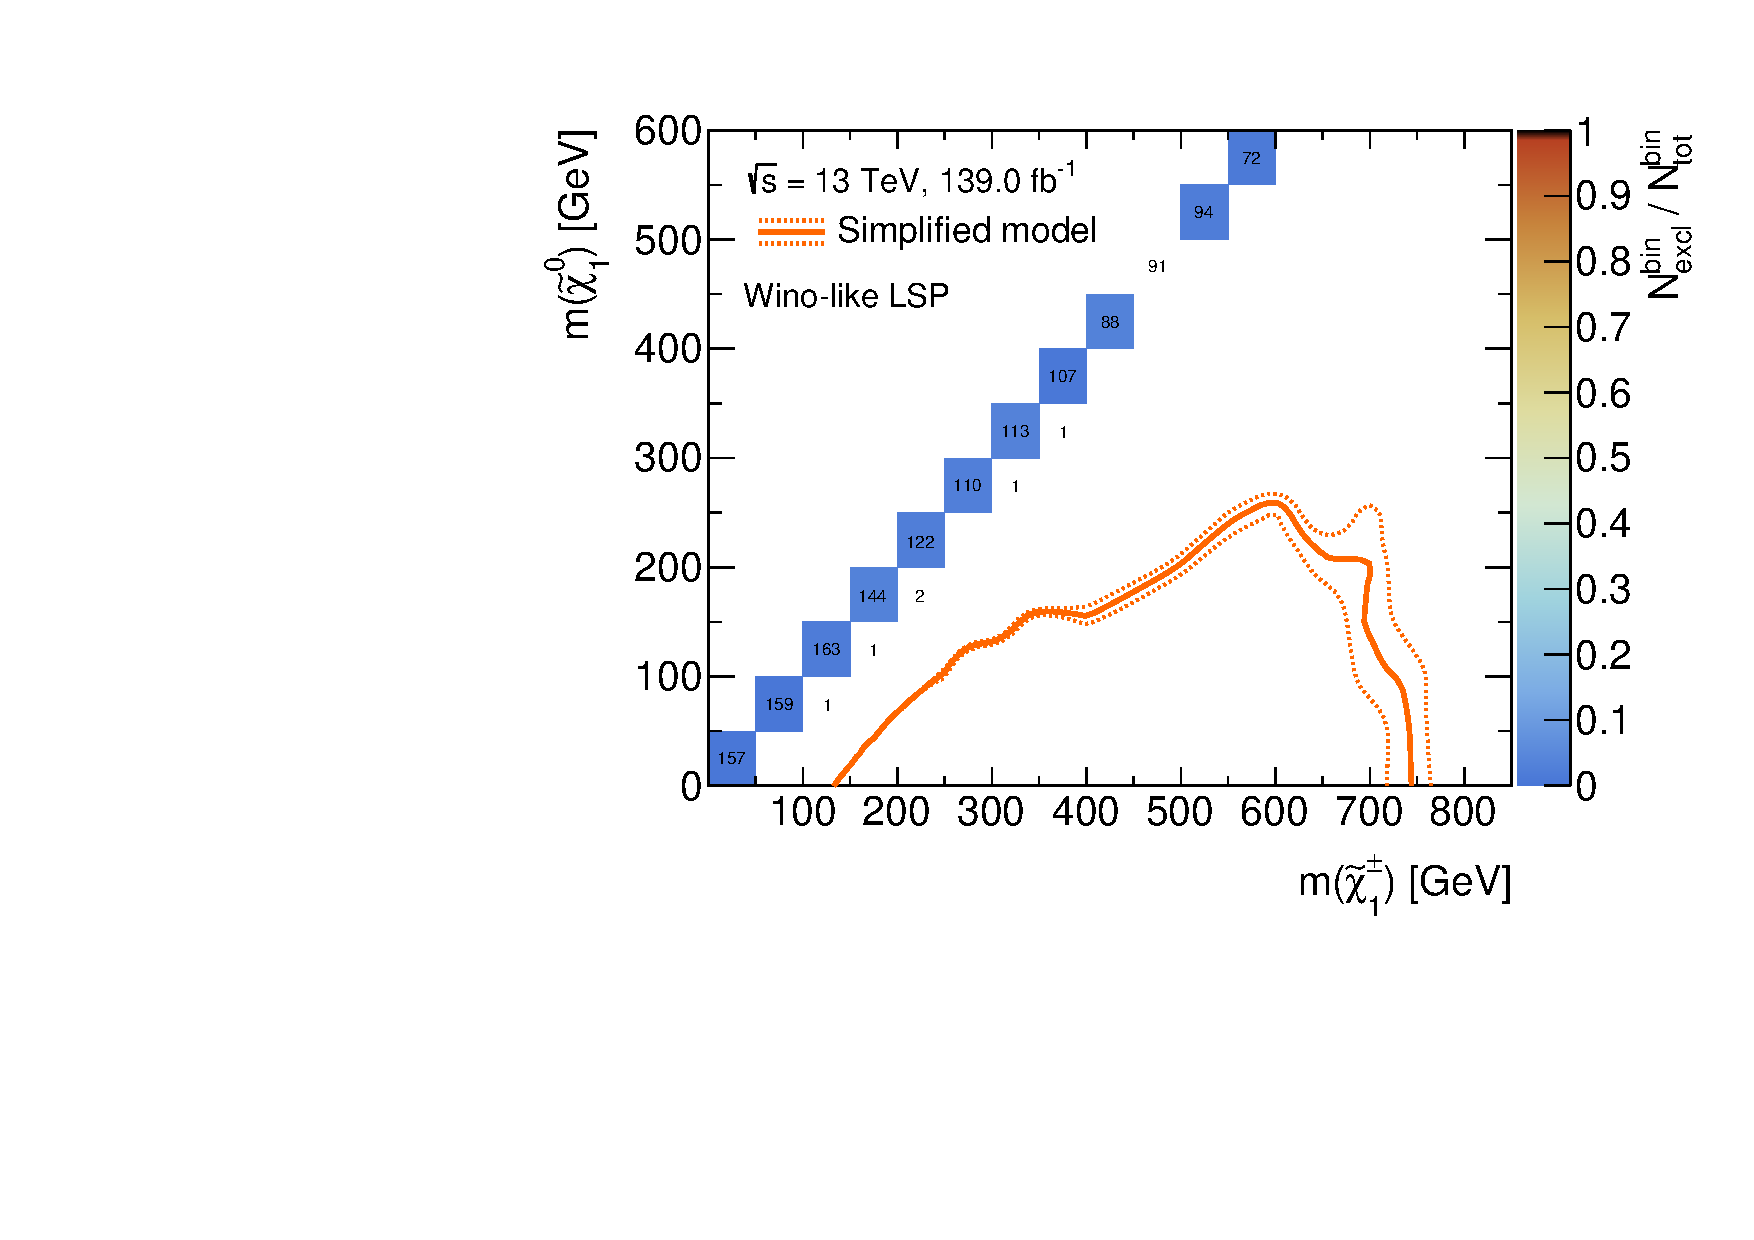
\includegraphics[width=\textwidth]{cut_wino_LSP/mchi1p_mlsp_contour}
%		\caption{\label{fig:mchi1p_mlsp_contour_wino_lsp}}
%	\end{subfigure}\hfill
%	\begin{subfigure}[b]{0.5\linewidth}
%		\centering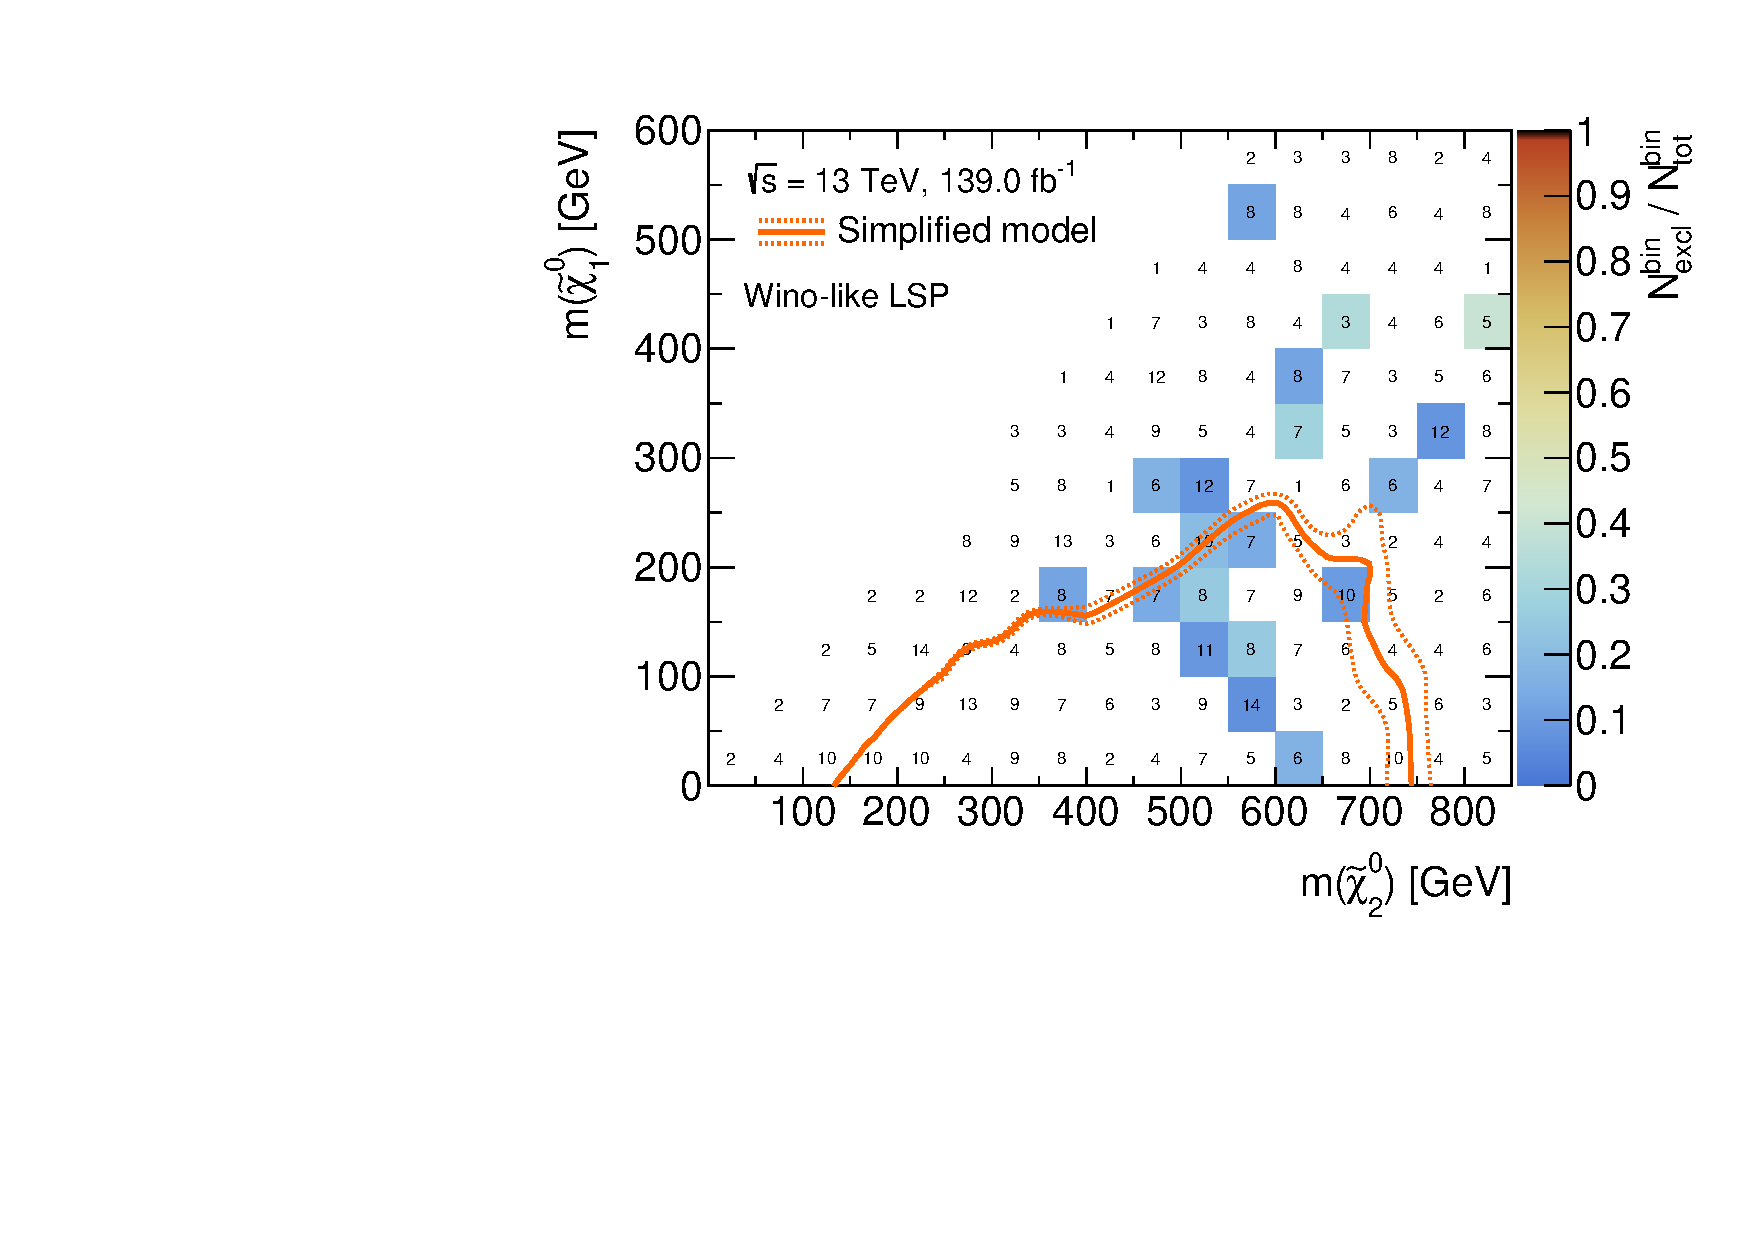
\includegraphics[width=\textwidth]{cut_wino_LSP/mchi20_mlsp_contour}
%		\caption{\label{fig:mchi20_mlsp_contour_wino_lsp}}
%	\end{subfigure}\hfill
%	\begin{subfigure}[b]{0.5\linewidth}
%		\centering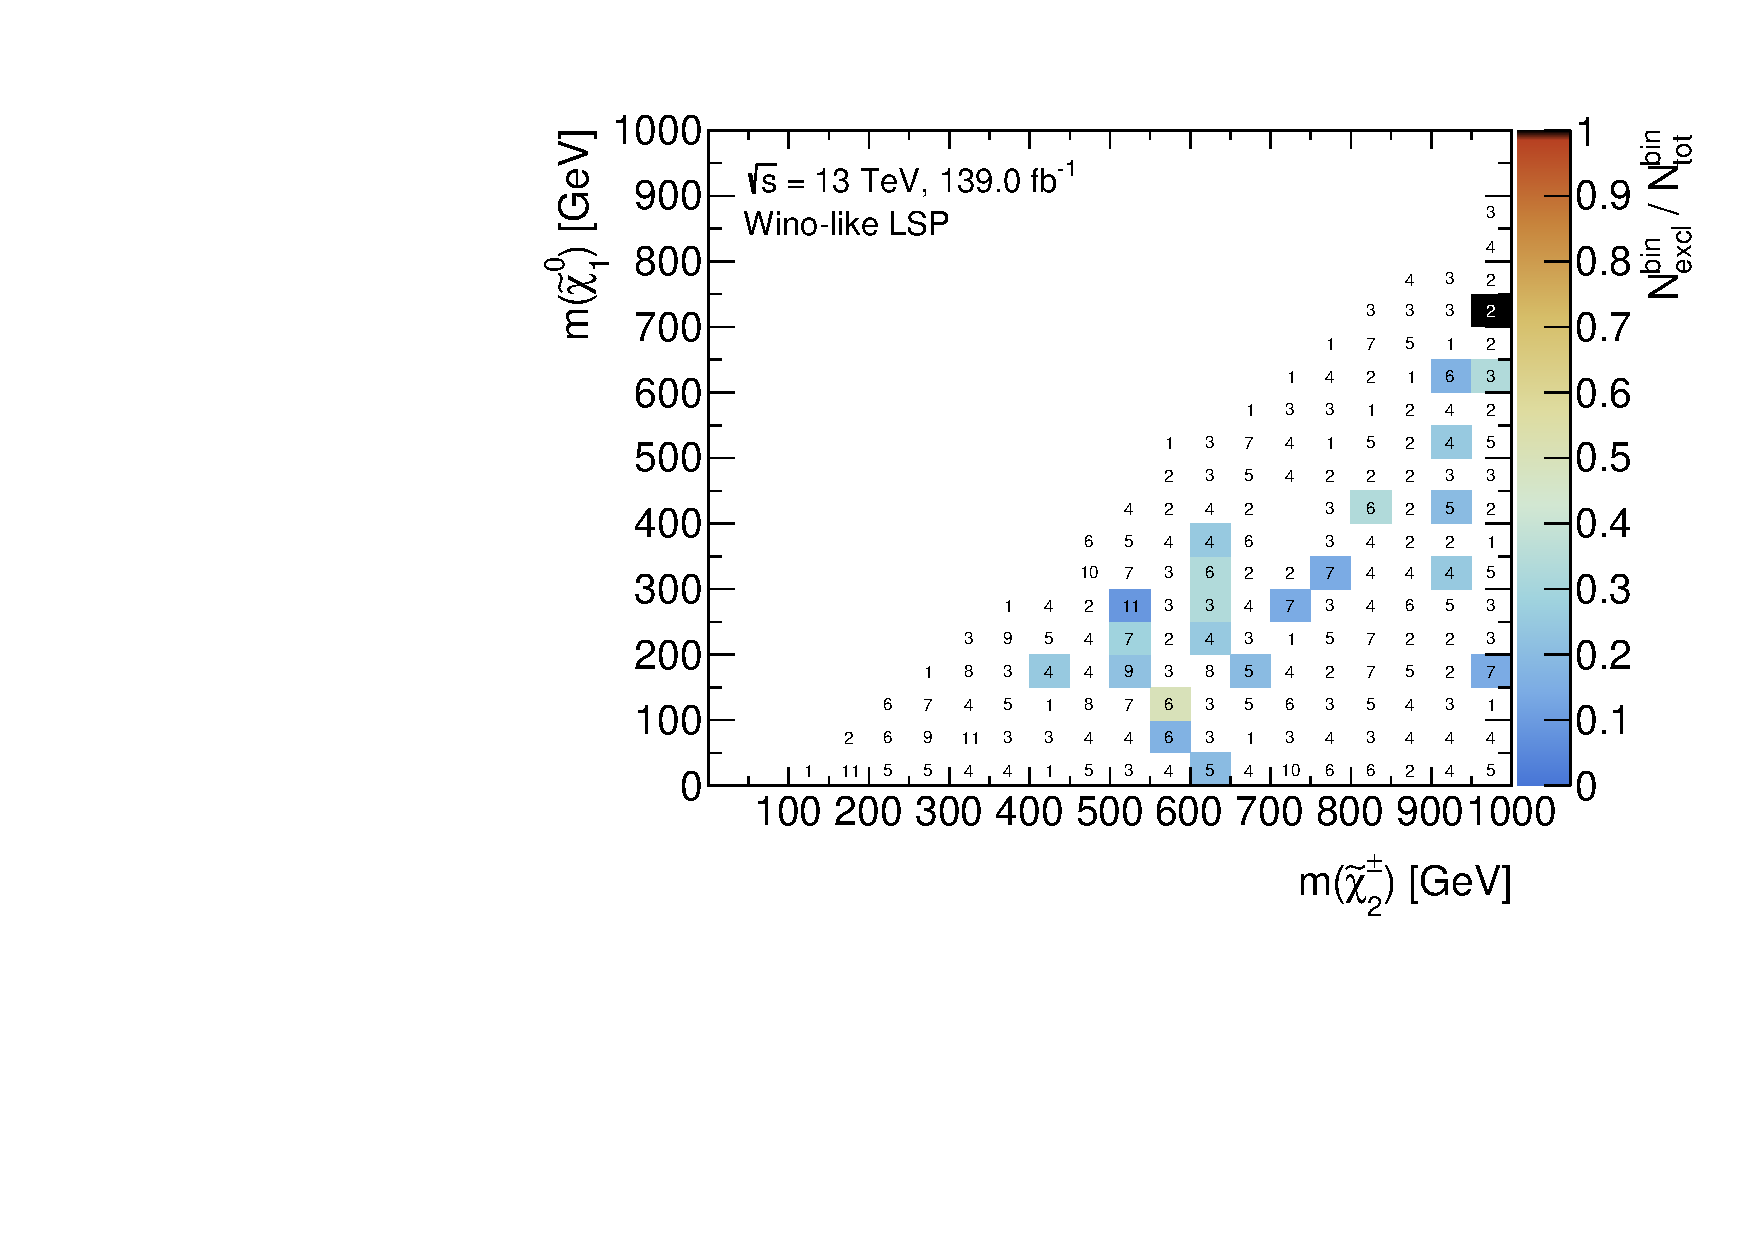
\includegraphics[width=\textwidth]{cut_wino_LSP/mchi10_mchi2p_contour}
%		\caption{\label{fig:mchi10_mchi2p_contour_wino_lsp}}
%	\end{subfigure}\hfill
%	\caption{Bin-by-bin fraction of excluded models as a function of the relevant sparticle masses. Only \gls{pmssm} models with a wino-like \gls{lsp} are shown. The numbers in the bins correspond to the total number of models sampled falling into the respective bin. The number of models excluded by the 1-lepton analysis is encoded with a colour bar ranging from 0 to 1. Where all models in a given bin are excluded, the bin is coloured in black. Bins without a models excluded are left white. Models are evaluated using the simplified likelihood of the 1-lepton analysis. The simplified model contour is shown in orange.}
%	\label{fig:impact_electroweakinos_2D_wino_lsp}
%\end{figure}

% \begin{figure}
%	\centering
%	\begin{subfigure}[b]{0.5\linewidth}
%		\centering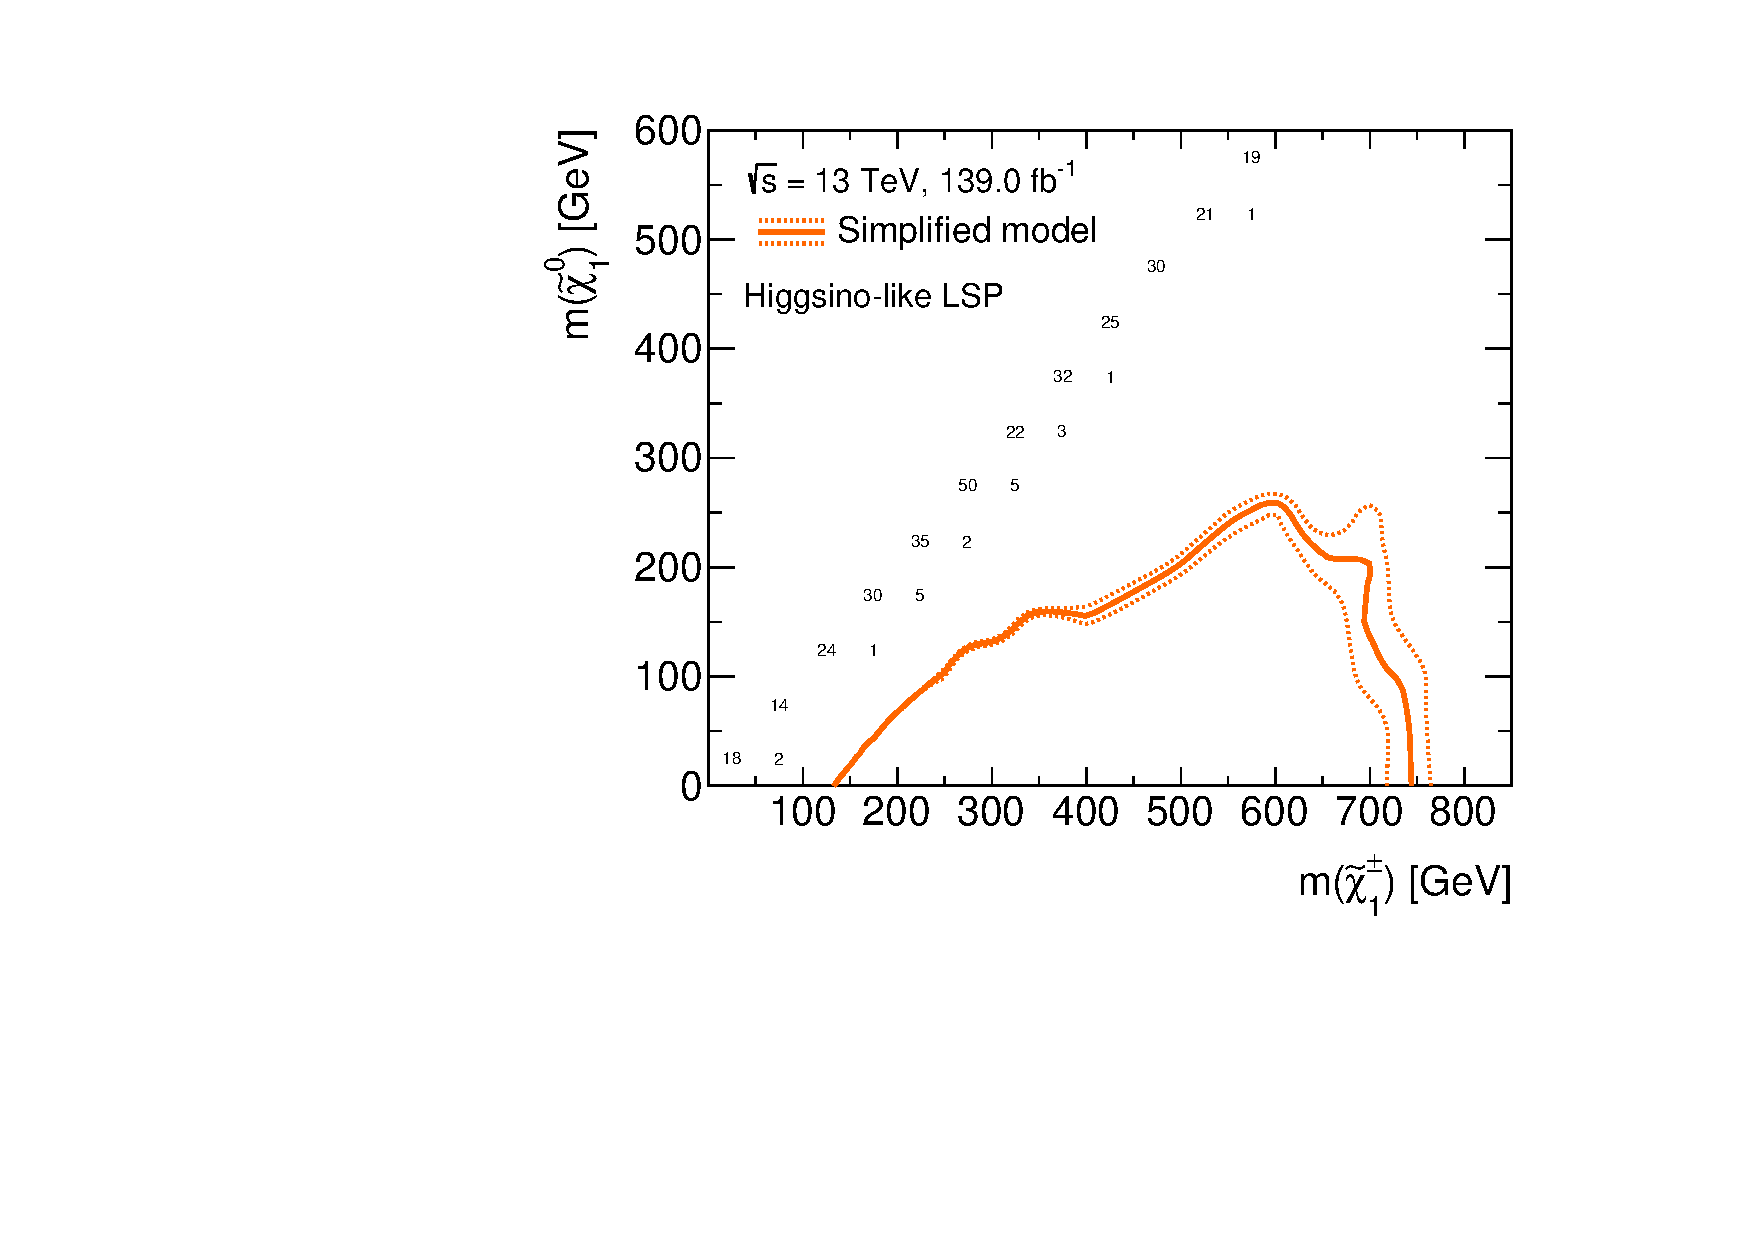
\includegraphics[width=\textwidth]{cut_higgsino_LSP/mchi1p_mlsp_contour}
%		\caption{\label{fig:mchi1p_mlsp_contour_higgsino_lsp}}
%	\end{subfigure}\hfill
%	\begin{subfigure}[b]{0.5\linewidth}
%		\centering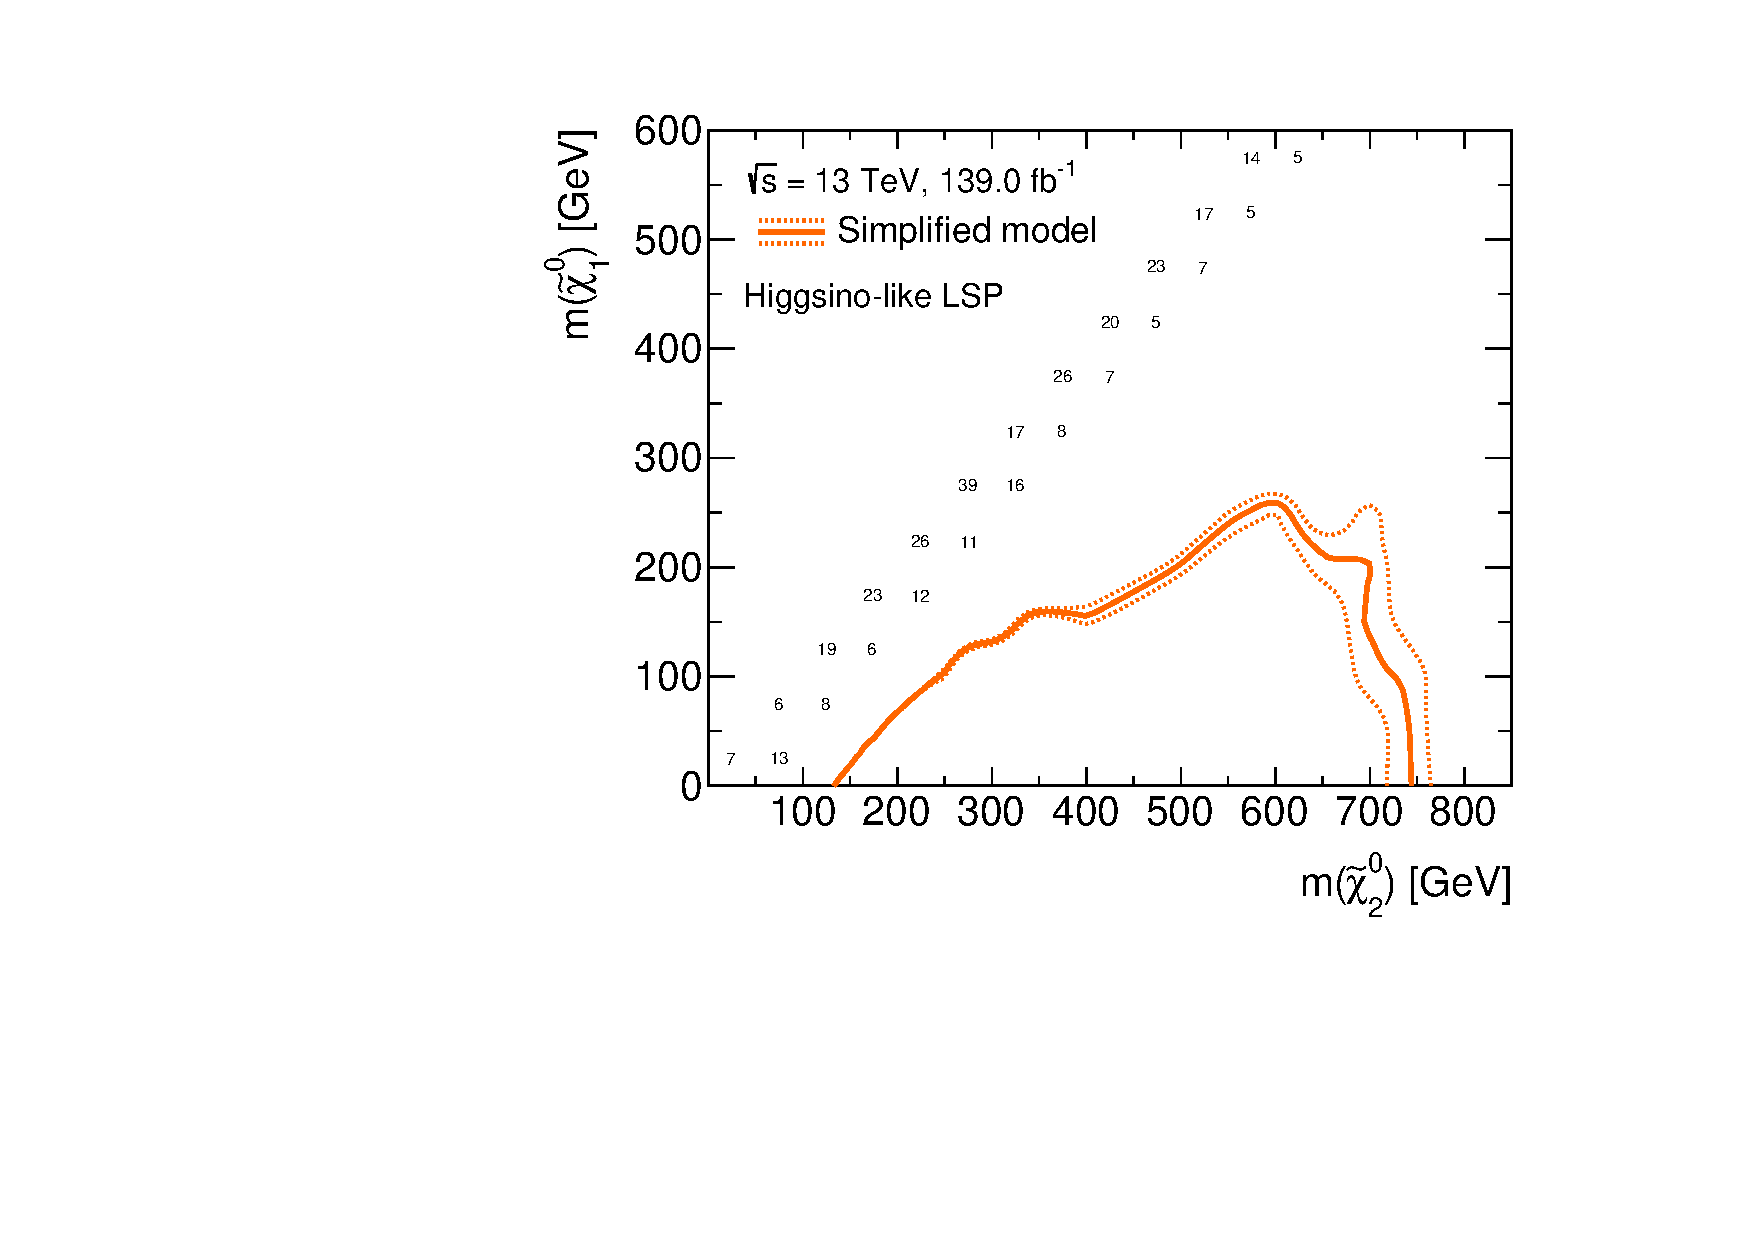
\includegraphics[width=\textwidth]{cut_higgsino_LSP/mchi20_mlsp_contour}
%		\caption{\label{fig:mchi20_mlsp_contour_higgsino_lsp}}
%	\end{subfigure}\hfill
%	\begin{subfigure}[b]{0.5\linewidth}
%		\centering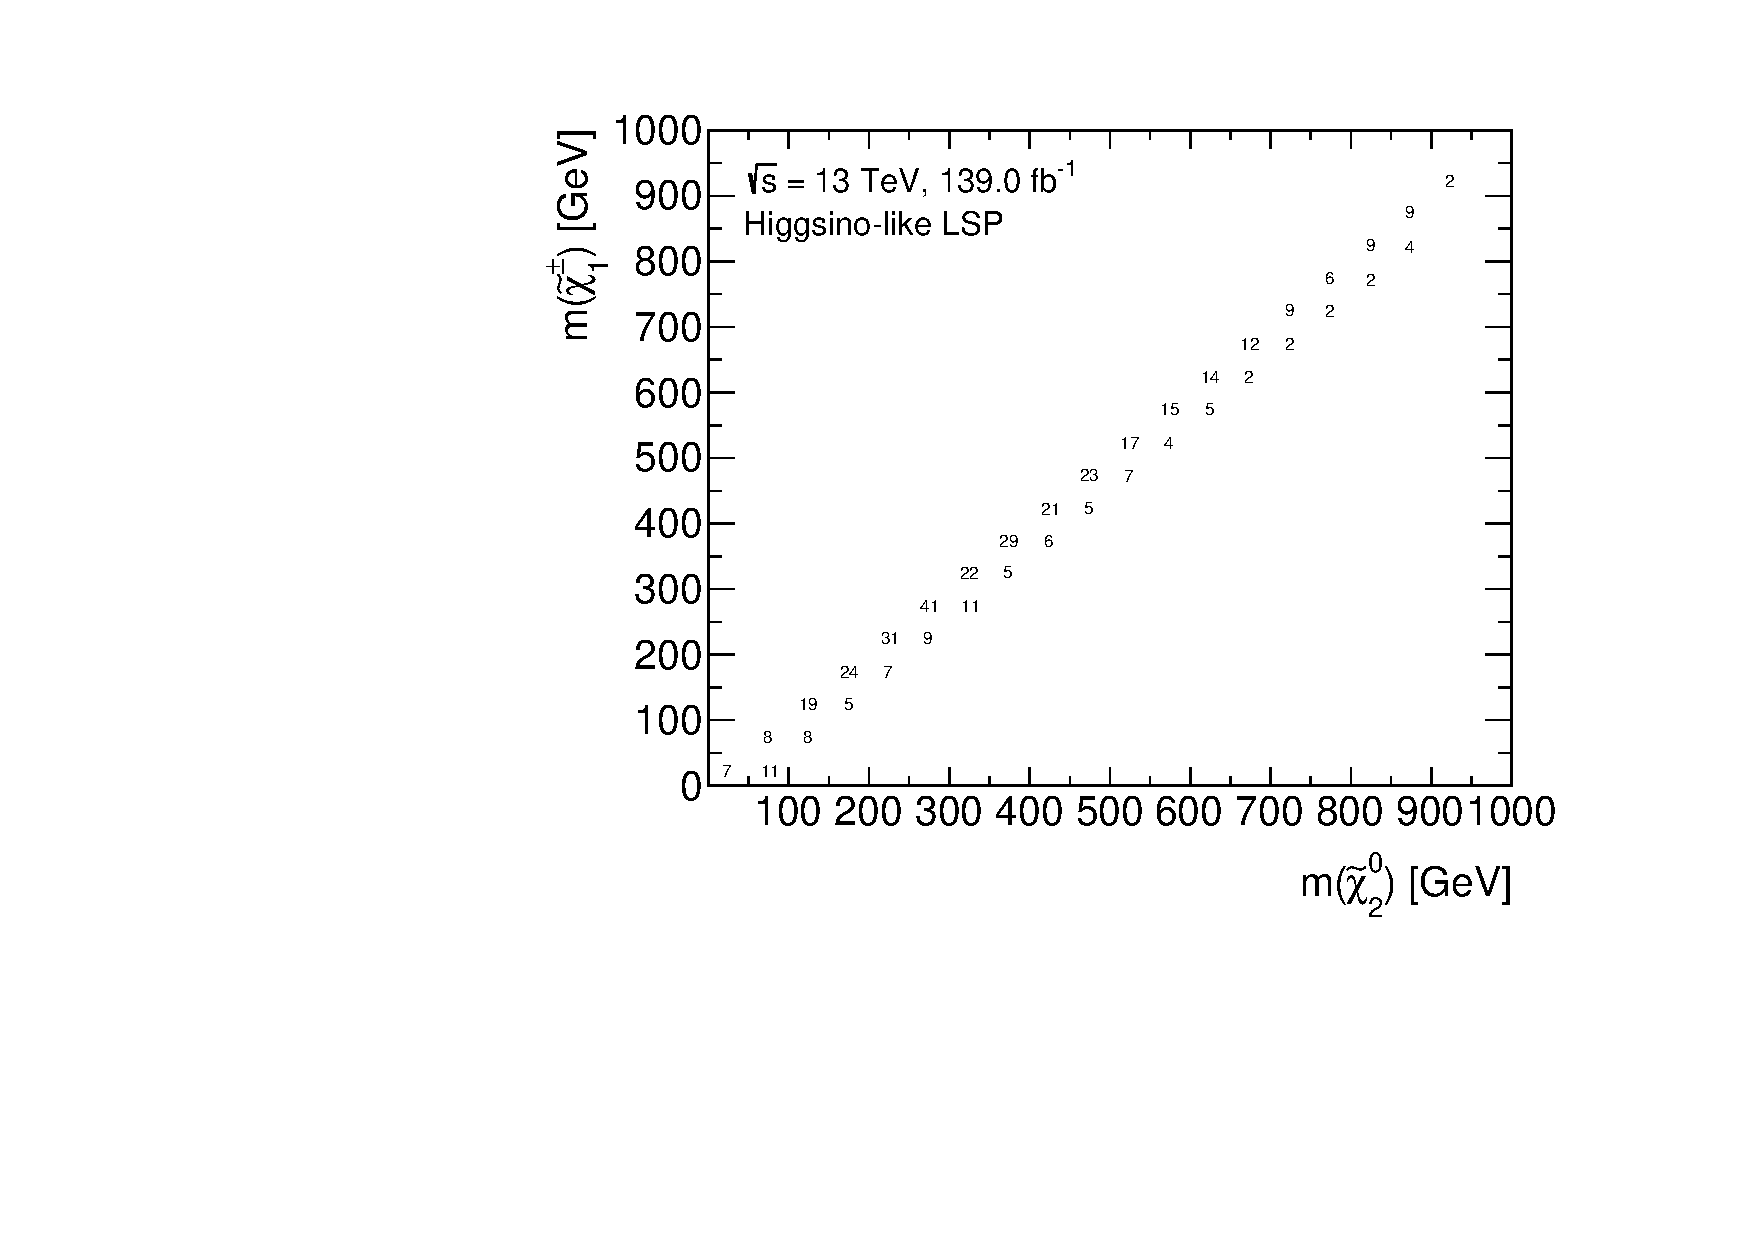
\includegraphics[width=\textwidth]{cut_higgsino_LSP/mchi1p_mchi20_contour}
%		\caption{\label{fig:mchi1p_mchi20_contour_higgsino_lsp}}
%	\end{subfigure}\hfill
%	\caption{Bin-by-bin fraction of excluded models as a function of the relevant sparticle masses. Only \gls{pmssm} models with a higgsino-like \gls{lsp} are shown. The numbers in the bins correspond to the total number of models sampled falling into the respective bin. The number of models excluded by the 1-lepton analysis is encoded with a colour bar ranging from 0 to 1. Where all models in a given bin are excluded, the bin is coloured in black. Bins without a models excluded are left white. Models are evaluated using the simplified likelihood of the 1-lepton analysis. The simplified model contour is shown in orange.}
%	\label{fig:impact_electroweakinos_2D_higgsino_lsp}
%\end{figure}


\FloatBarrier

\section{Higgs coupling to neutralinos}

The couplings of the $\neutr$ to the Higgs boson are suppressed by powers of $\vert\mu\vert/M_2$ in the wino-like and bino-like scnearios~\cite{Arbey:2012fa}, meaning that the branching fraction of $\neutr \rightarrow h \lsp$ takes on reasonably high values only in models with an \gls{lsp} that is nearly pure bino. The suppression behaviour is illustrated in \cref{fig:higgs_coupling_neutralino}.

\begin{figure}[h]
	\centering
	\begin{subfigure}[b]{0.49\linewidth}
		\centering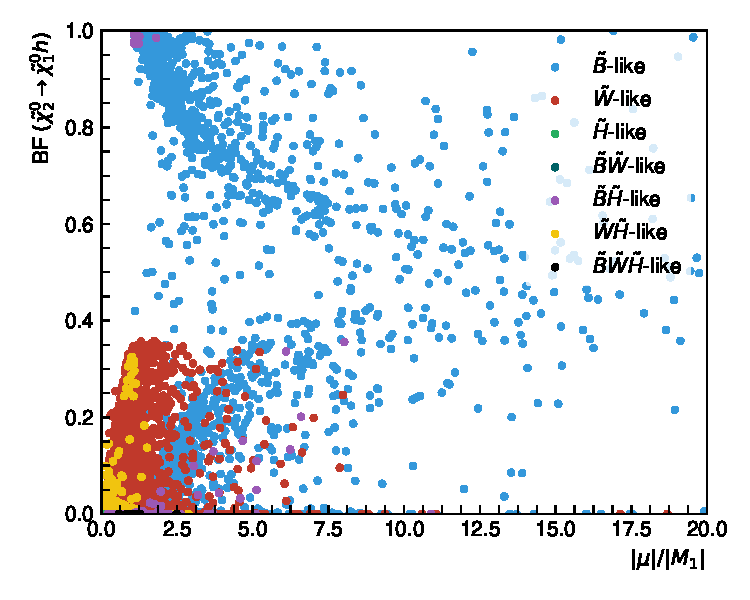
\includegraphics[width=\textwidth]{scatter/lsp_types_BR_Higgs_muM1}
		\caption{\label{fig:lsp_types_BR_Higgs_muM1}}
	\end{subfigure}\hfill
	\begin{subfigure}[b]{0.49\linewidth}
		\centering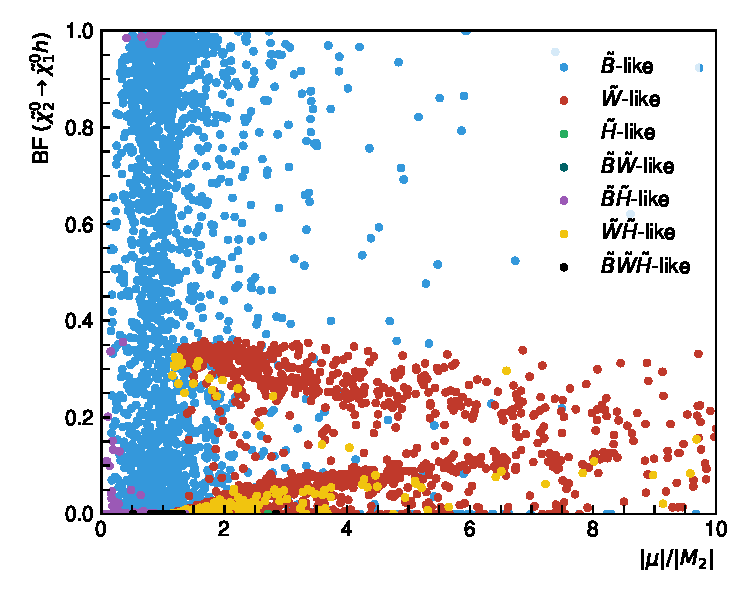
\includegraphics[width=\textwidth]{scatter/lsp_types_BR_Higgs_muM2}
		\caption{\label{fig:lsp_types_BR_Higgs_muM2}}
	\end{subfigure}\hfill
	\caption{Density of the \gls{pmssm} models projected onto the plane spanned by $\mathrm{BF}(\neutr \rightarrow h \lsp)$ and \subref{fig:lsp_types_BR_Higgs_muM1} $\vert\mu\vert/\vert M_1 \vert$ or \subref{fig:lsp_types_BR_Higgs_muM2} $\vert\mu\vert/\vert M_2 \vert$. Models are shown as a function of their $\lsp$ type.}
	\label{fig:higgs_coupling_neutralino}
\end{figure}

\FloatBarrier

\section{Impact on pMSSM parameters}

In \cref{fig:impact_pMSSM_parameters_1D_2}, the impact of the \onelepton search on the reminaing \gls{pmssm} parameters sampled, not already shown in \cref{sec:impact_pmssm_parameters}, are provided. As before, the full set of models evaluated with the \onelepton search is shown as black line, while the bin-wise number of models excluded by the search are indicated with the blue histogram. An additional pad indicates the fraction of models excluded in each bin.

\begin{figure}
	\centering
	\begin{subfigure}[b]{0.4\linewidth}
		\centering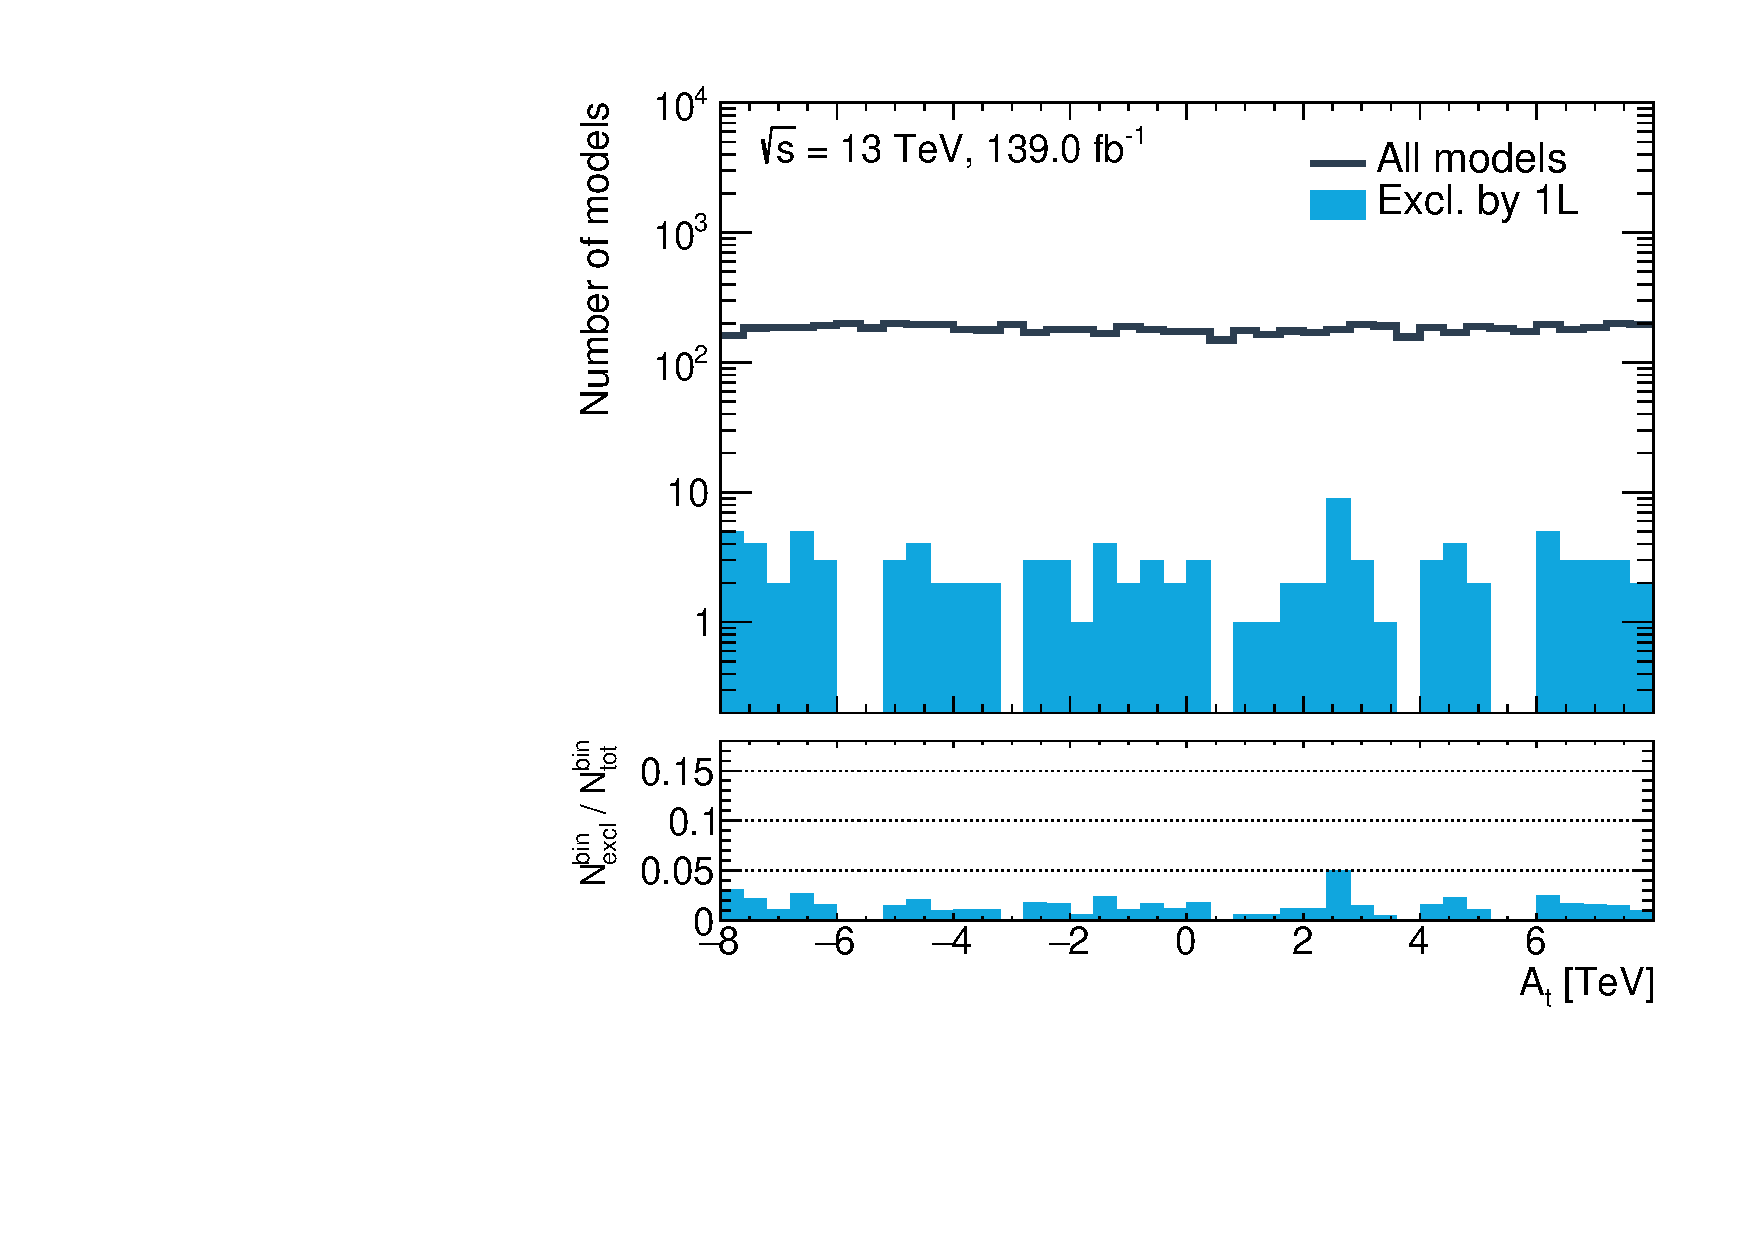
\includegraphics[width=\textwidth]{1D/At}
	\end{subfigure}
	\begin{subfigure}[b]{0.4\linewidth}
		\centering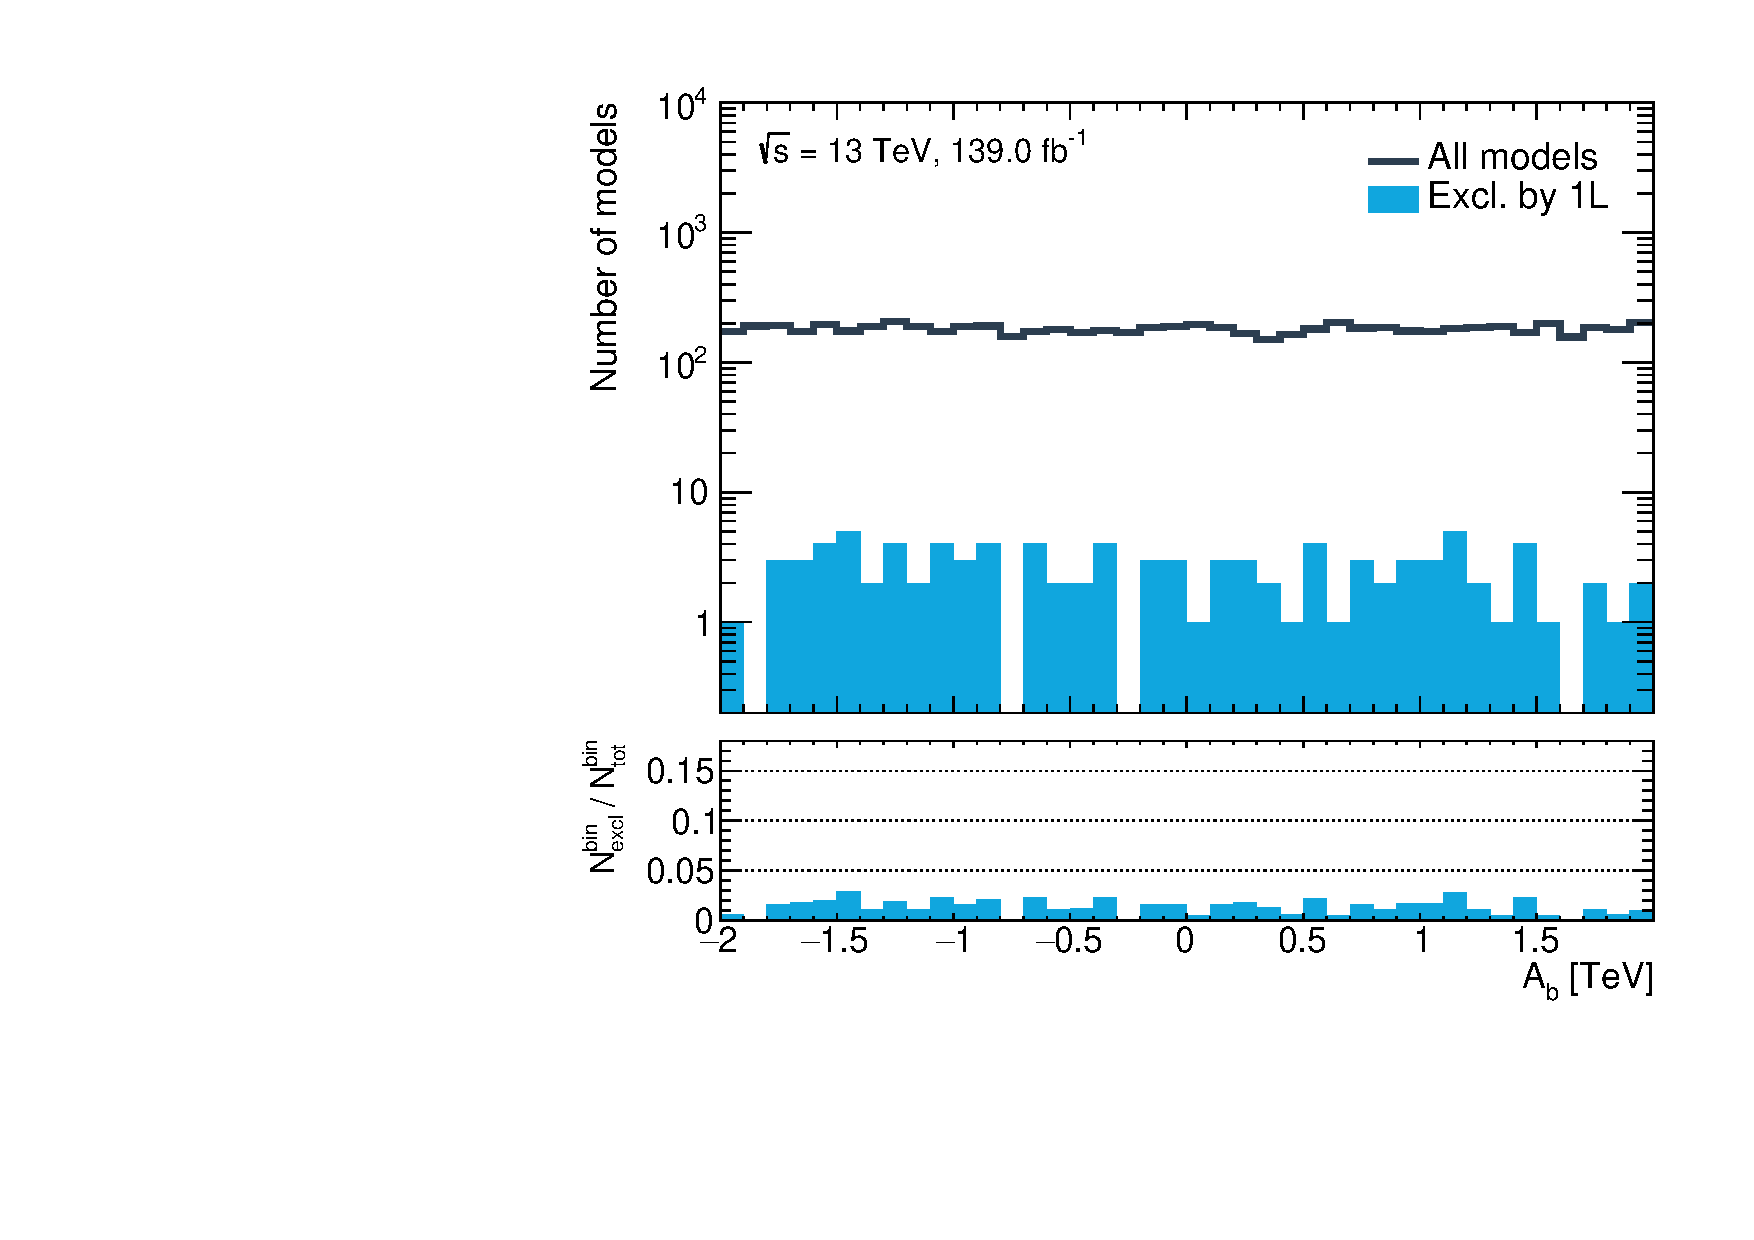
\includegraphics[width=\textwidth]{1D/Ab}
	\end{subfigure}
	\begin{subfigure}[b]{0.4\linewidth}
		\centering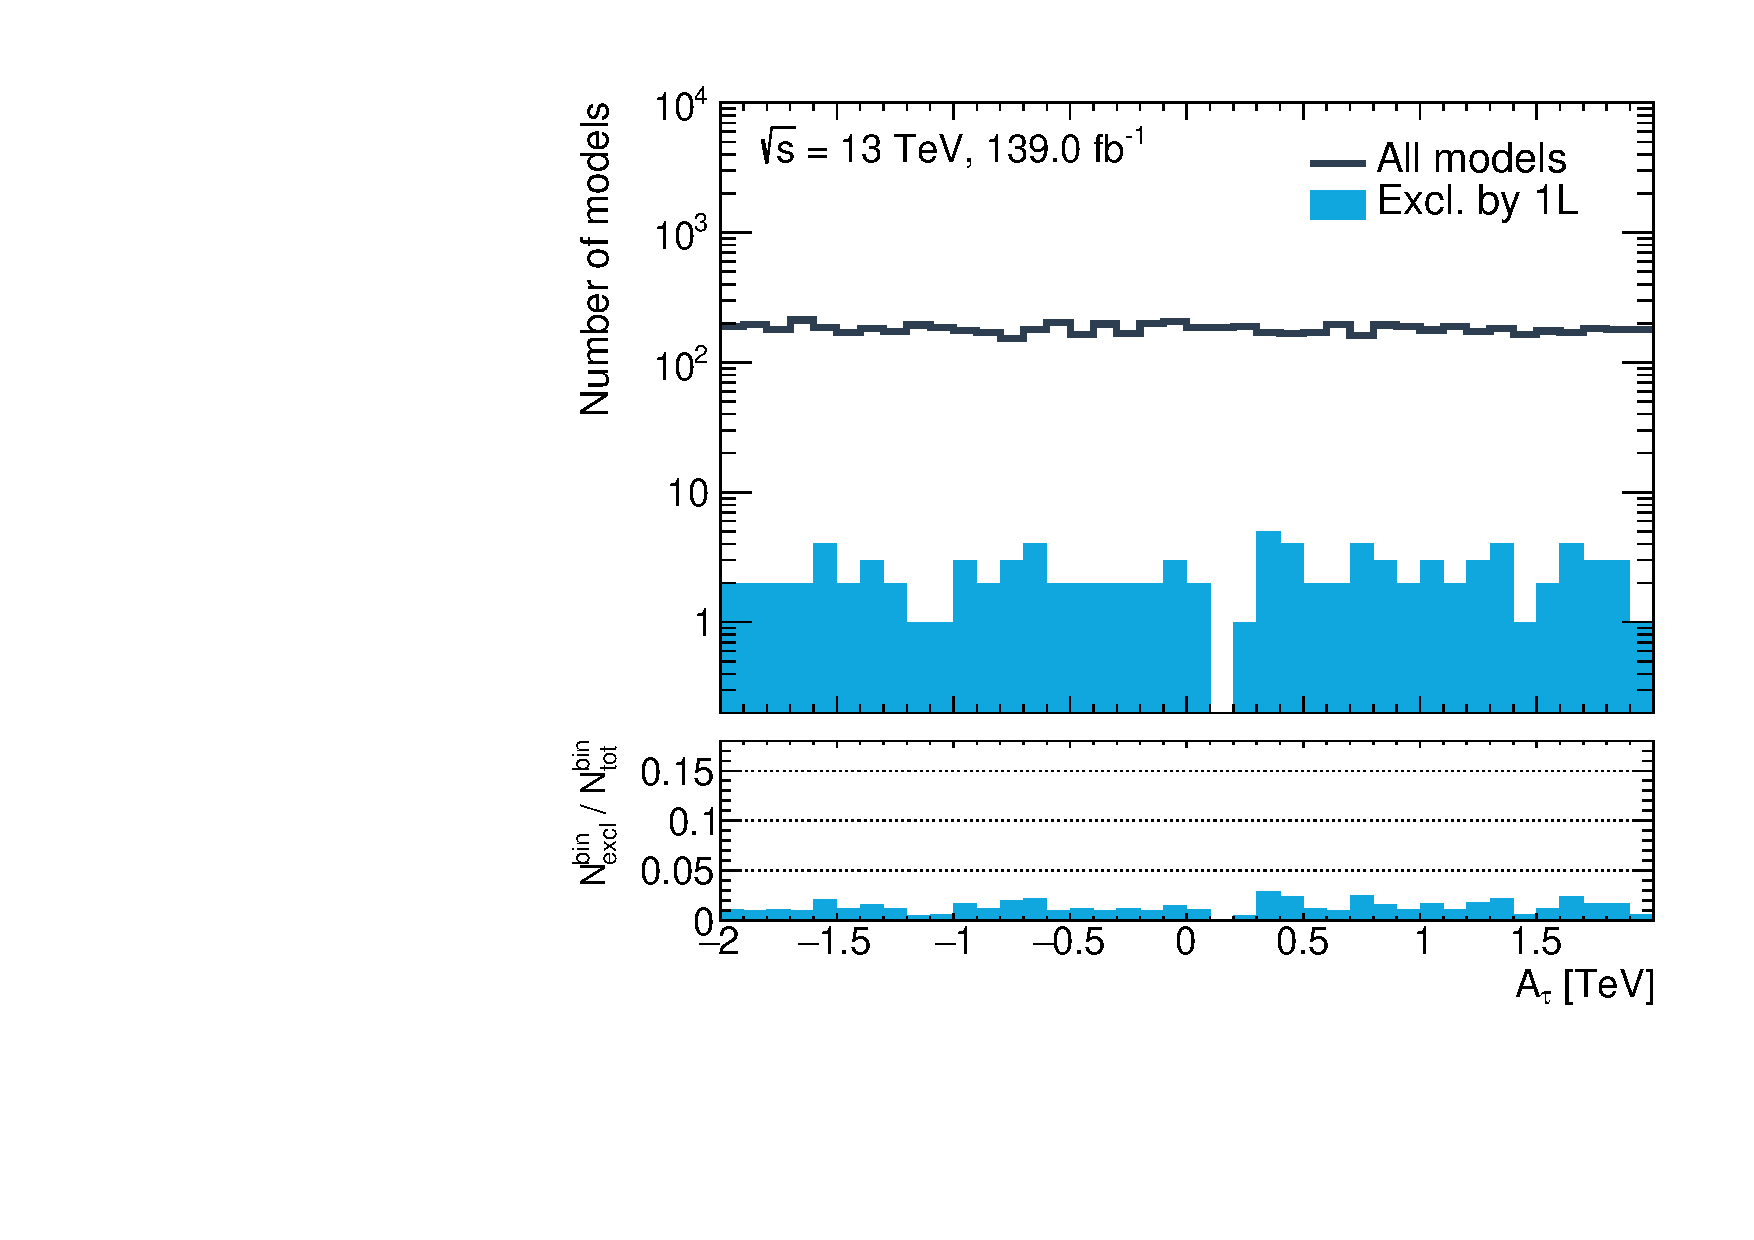
\includegraphics[width=\textwidth]{1D/Atau}
	\end{subfigure}
	\begin{subfigure}[b]{0.4\linewidth}
		\centering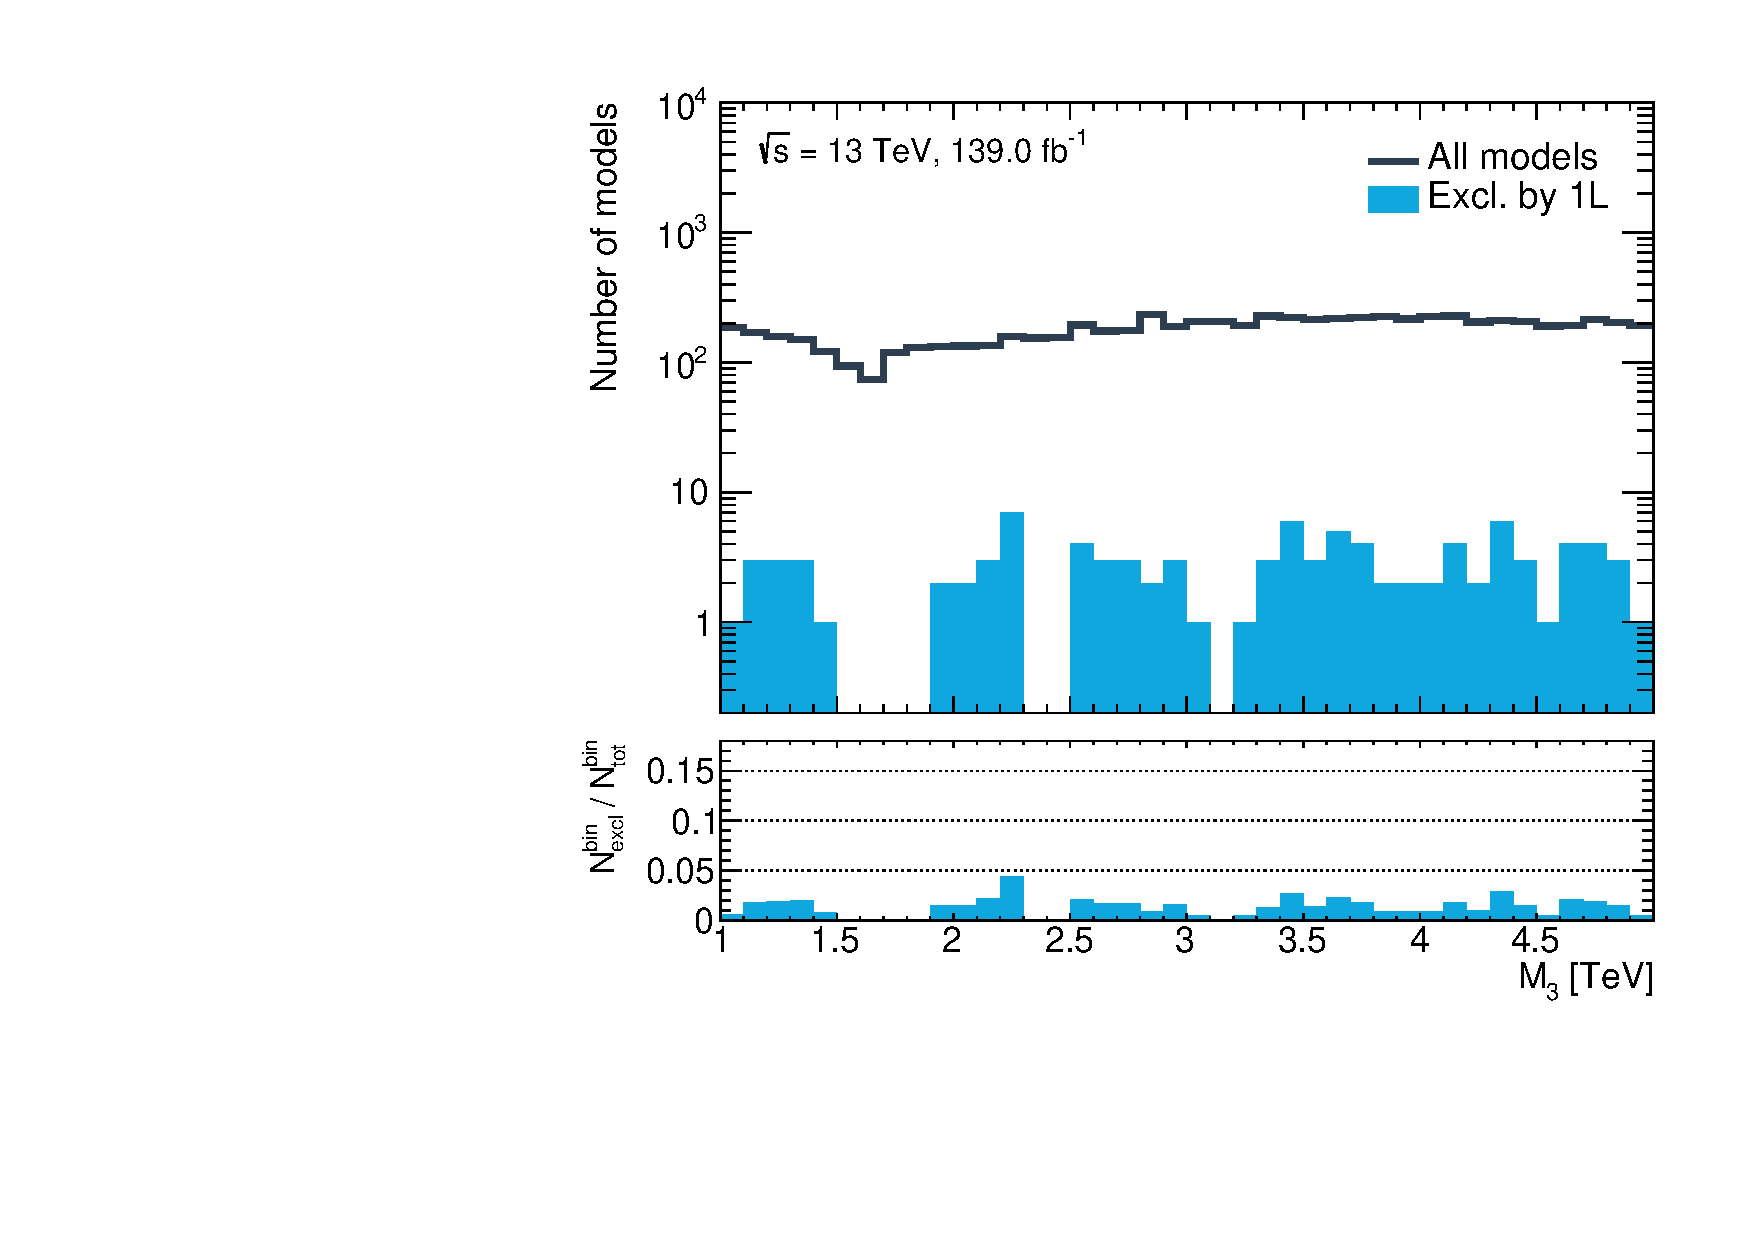
\includegraphics[width=\textwidth]{1D/M3}
	\end{subfigure}
	\begin{subfigure}[b]{0.4\linewidth}
		\centering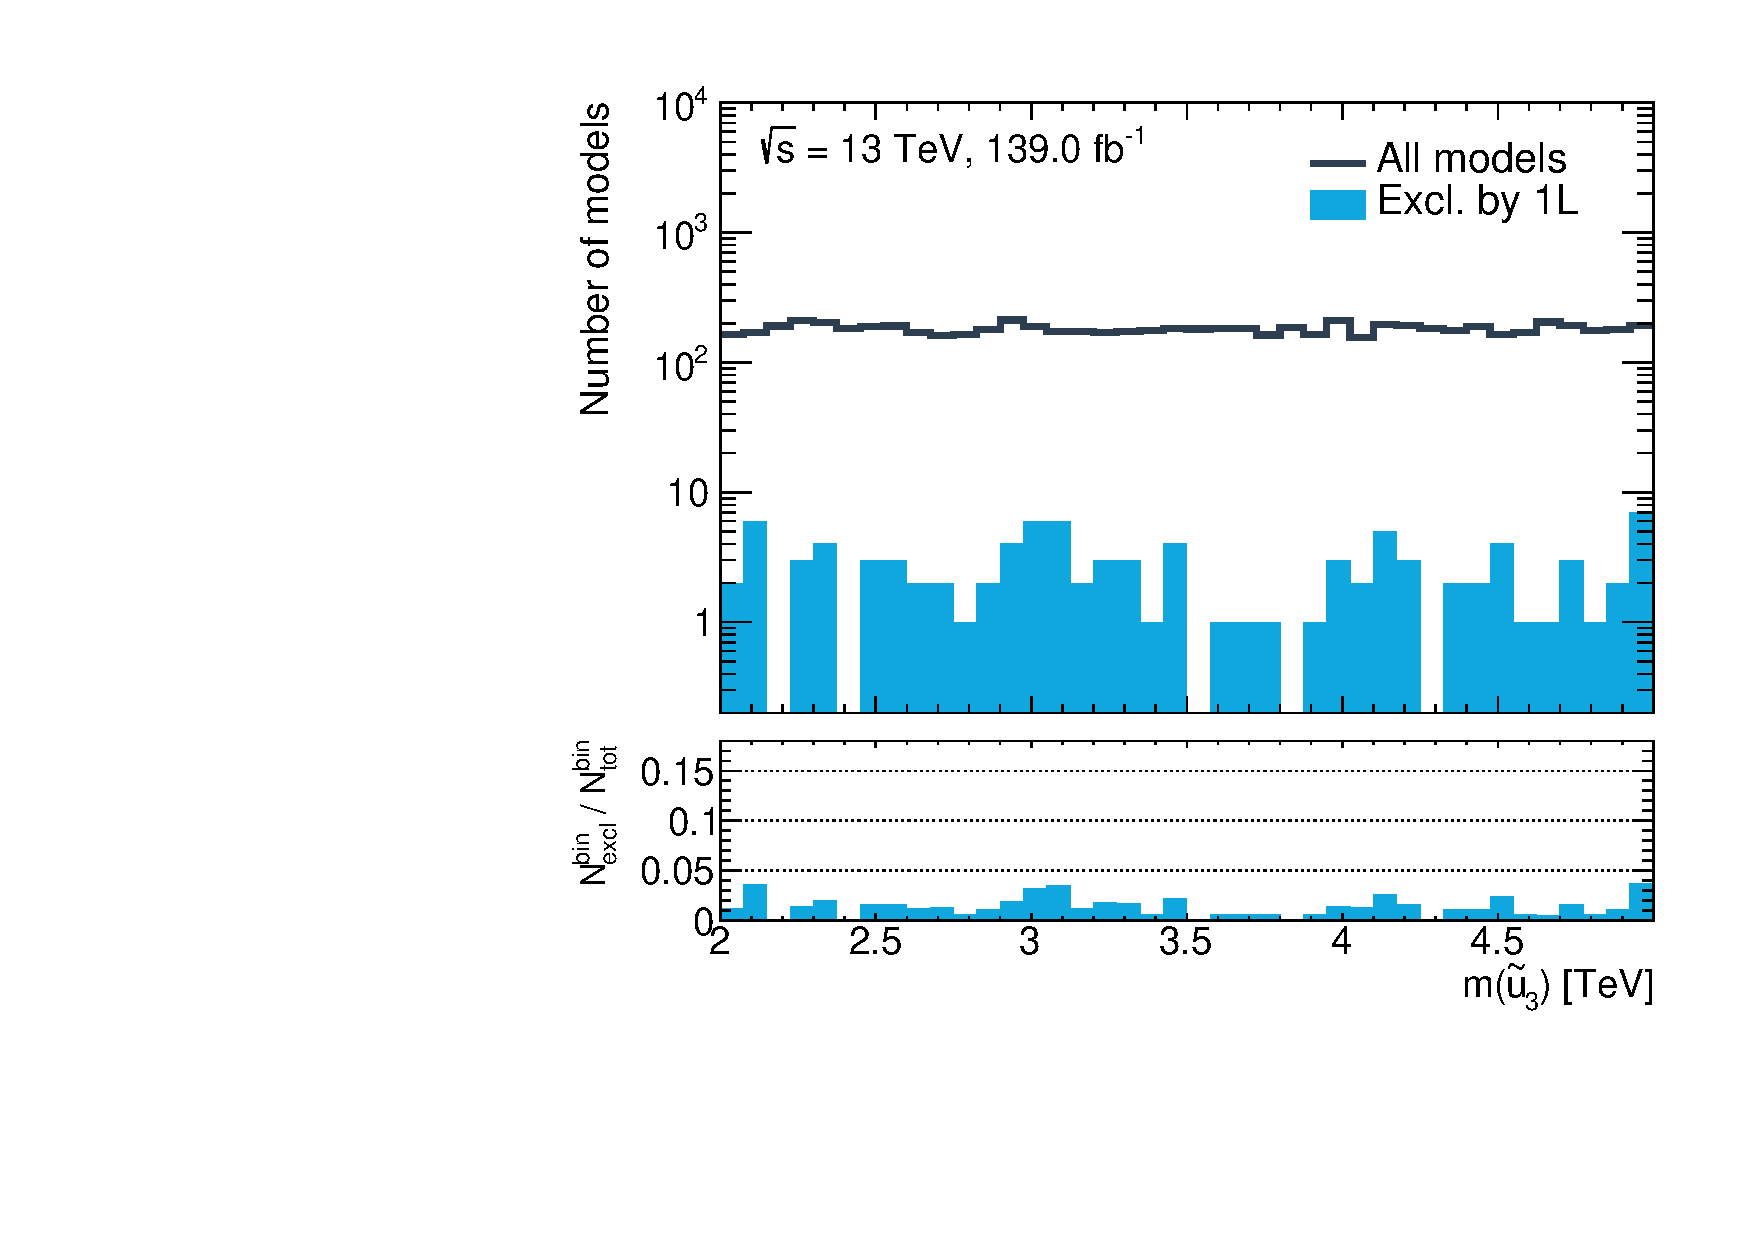
\includegraphics[width=\textwidth]{1D/mtR}
	\end{subfigure}
	\begin{subfigure}[b]{0.4\linewidth}
		\centering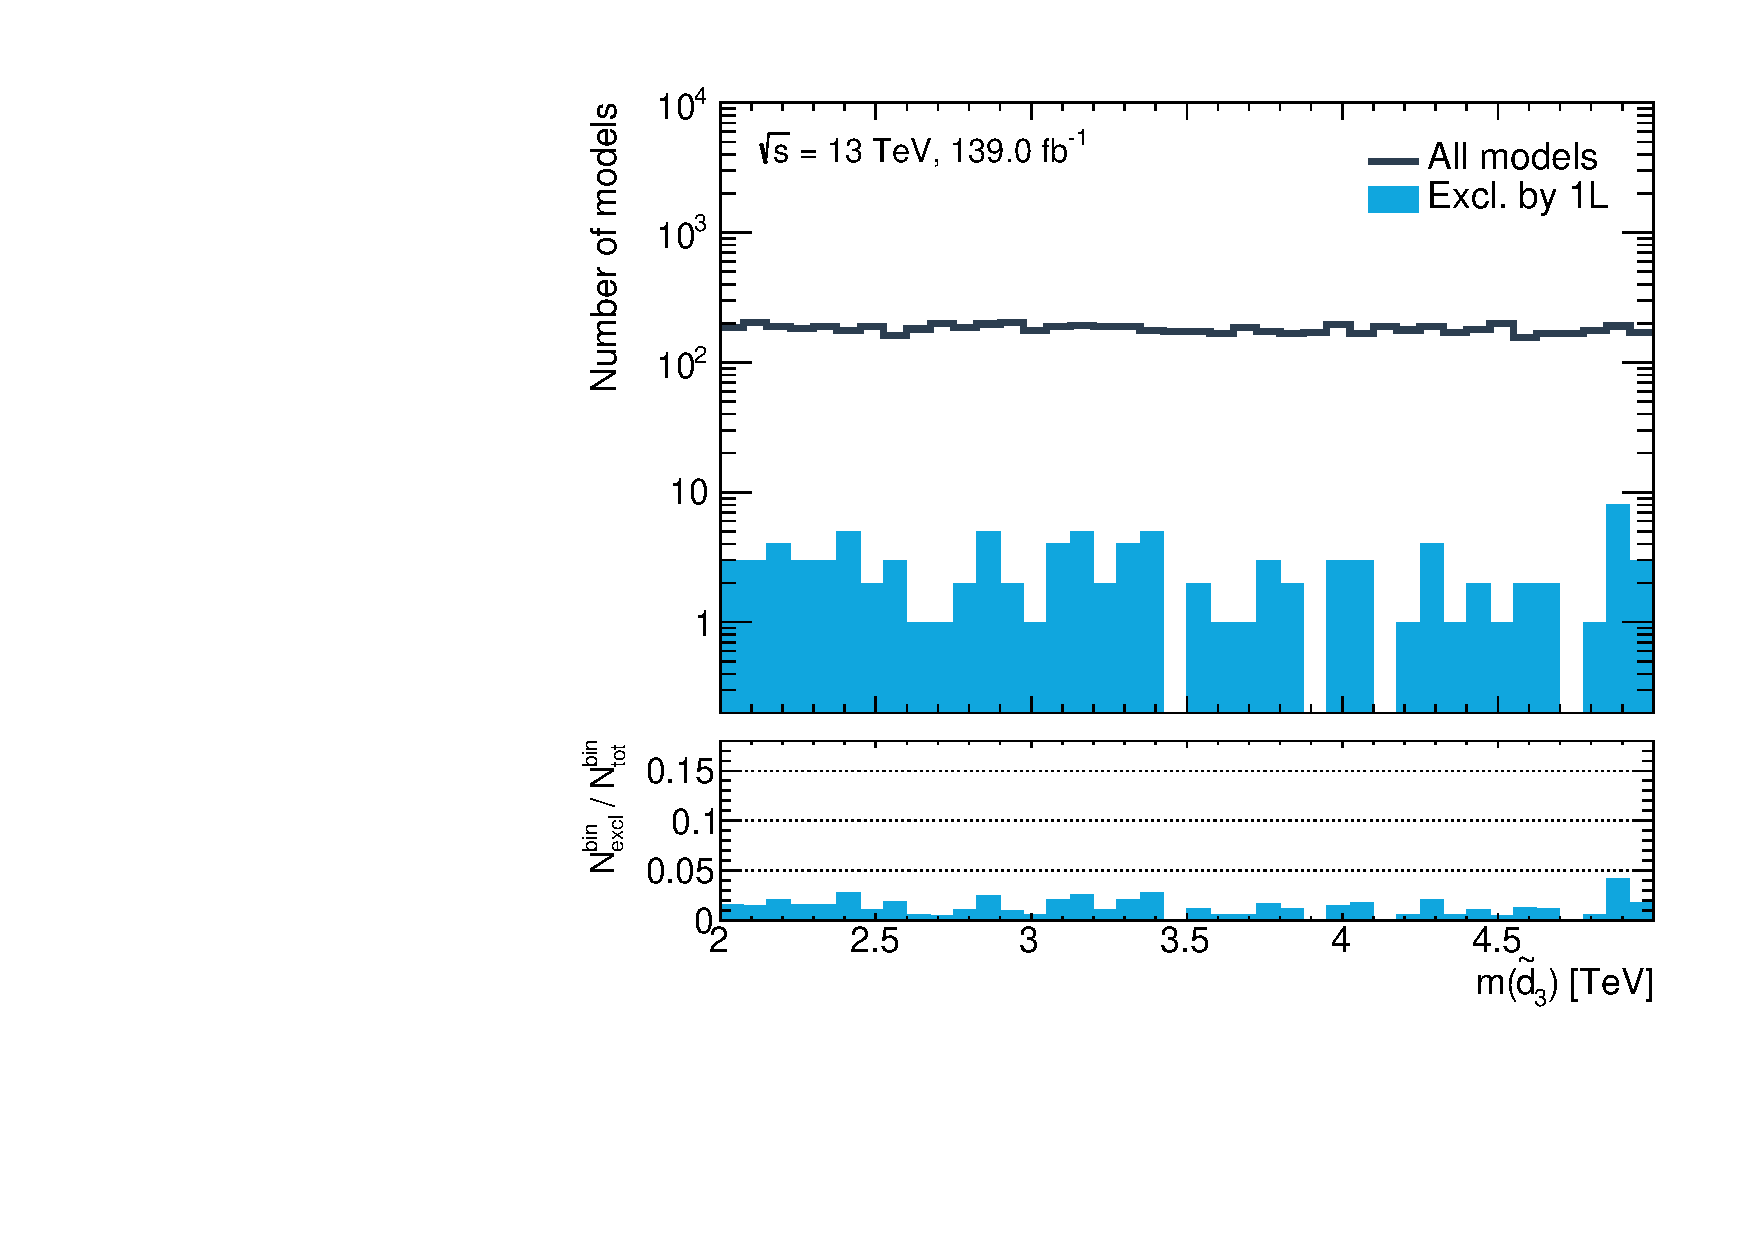
\includegraphics[width=\textwidth]{1D/mbR}
	\end{subfigure}
	\begin{subfigure}[b]{0.4\linewidth}
		\centering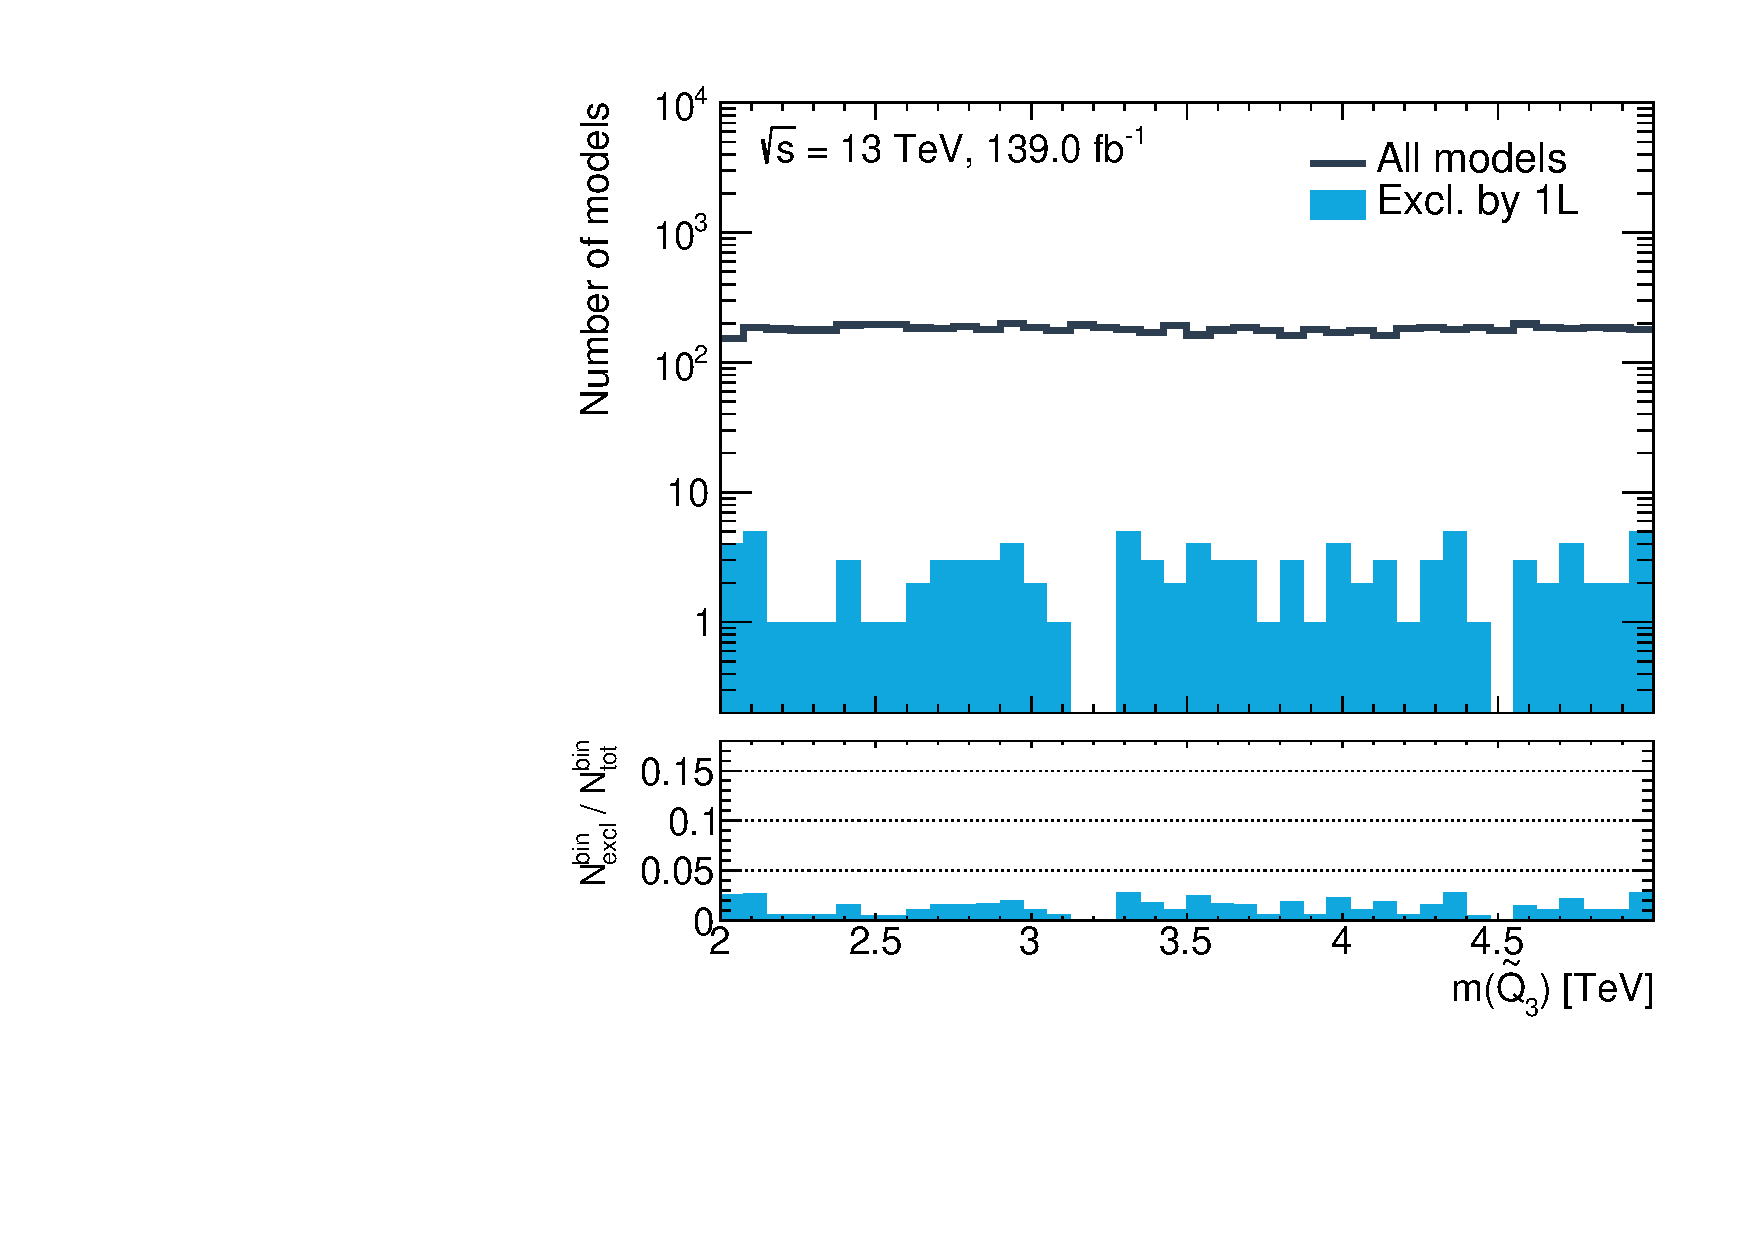
\includegraphics[width=\textwidth]{1D/mqL3}
	\end{subfigure}
	\caption{Bin-by-bin number of excluded models as a one-dimensional function of the remaining scanned \gls{pmssm} parameters not already shown in \cref{fig:impact_pMSSM_parameters_1D}. The bin-wise fraction of excluded models, $N^\mathrm{bin}_\mathrm{excl} / N^\mathrm{bin}_\mathrm{total}$, is shown in the lower pad. All models are evaluated using the simplified likelihood of the \onelepton search.}
	\label{fig:impact_pMSSM_parameters_1D_2}
\end{figure}


\FloatBarrier

\section{Impact on dark matter relic density}

\Cref{fig:relic_density_lsp_withConstraint} compares the density of \gls{pmssm} models in a two-dimensional projection on the $\Omega_{\tilde{\chi}} h^2$--$m(\lsp)$ plane before and after the \gls{lep} constraint on the chargino mass of $\charg > \SI{103.5}{\GeV}$~\cite{lep_susy_results} is applied.

\begin{figure}[h]
	\centering
	\begin{subfigure}[b]{0.49\linewidth}
		\centering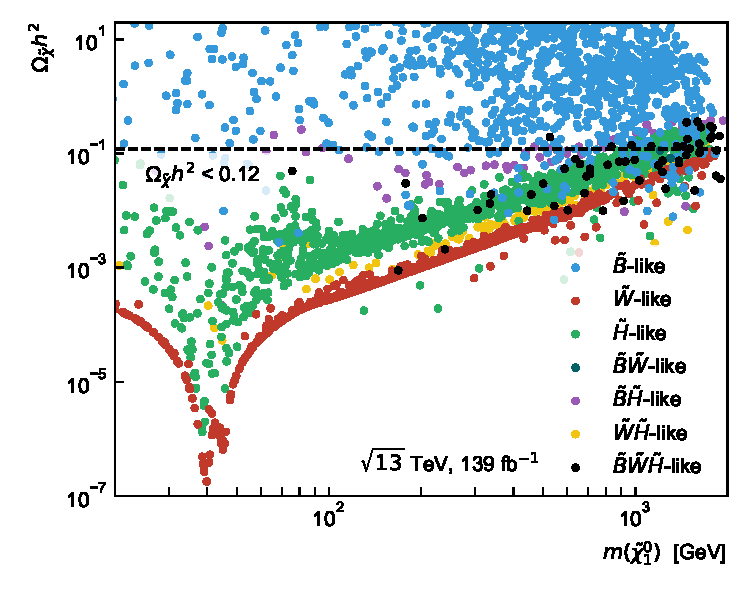
\includegraphics[width=\textwidth]{scatter/relic_density_lsp}
		\caption{\label{fig:relic_density_lsp_no_constraint}}
	\end{subfigure}\hfill
	\begin{subfigure}[b]{0.49\linewidth}
		\centering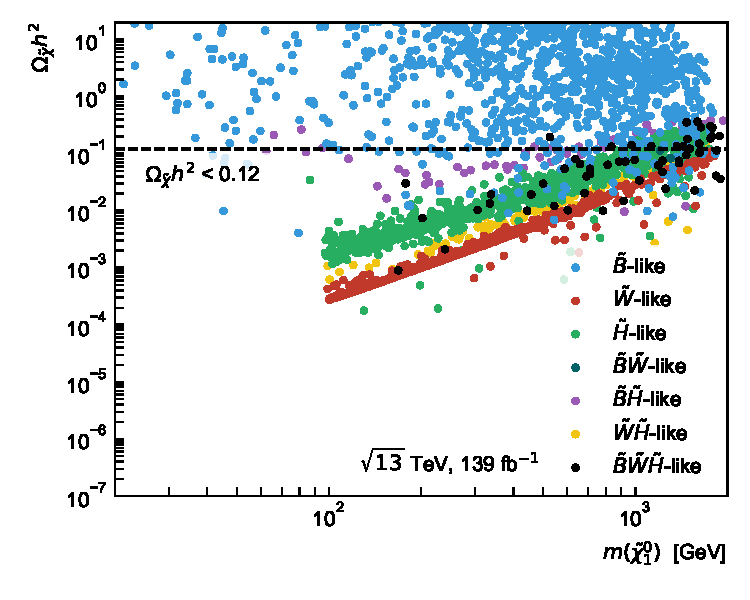
\includegraphics[width=\textwidth]{scatter/relic_density_lsp_limits}
		\caption{\label{fig:relic_density_lsp_constraint}}
	\end{subfigure}\hfill
	\caption{Density of the \gls{pmssm} model points sampled in the plane spanned by the relic density and the $\lsp$ mass. The model points are additionally shown as a function of the nature of their $\lsp$. In fig.~\subref{fig:relic_density_lsp_no_constraint} all \gls{pmssm} models originally sampled and evaluated are shown. In fig.~\subref{fig:relic_density_lsp_constraint}, only models satisfying the constraint $\charg > \SI{103.5}{\GeV}$ set by \gls{lep}~\cite{lep_susy_results} are shown. The horizontal dashed line represents the \gls{dm} relic density measurement by the Planck collaboration, interpreted as an upper limit $\Omega_{\tilde{\chi}} h^2 < 0.12$ such that the $\lsp$ can be a sub-dominant \gls{dm} component.}
	\label{fig:relic_density_lsp_withConstraint}
\end{figure}
